% ============================================================
%  BÁO CÁO TỔNG KẾT DỰ ÁN
%  Tối ưu hóa Pipe để Cải thiện Thông lượng IPC trong xv6
%  Operating Systems [Multimedia] -- 20252
%  Mã dự án: 25236
% ============================================================
\documentclass[12pt,a4paper]{article}

%% Encoding & language (XeLaTeX / LuaLaTeX -- UTF-8 natively, no inputenc/T5 needed)
\usepackage{fontspec}
\defaultfontfeatures{Ligatures=TeX}
\usepackage[vietnamese]{babel}

%% Layout
\usepackage[top=2.5cm, bottom=2.5cm, left=3cm, right=2.5cm, headheight=14pt]{geometry}
\usepackage{fancyhdr}
\pagestyle{fancy}
\fancyhf{}
%\fancyhead[L]{\small Operating Systems [Multimedia] -- 20252}
%\fancyhead[R]{\small Mã dự án: 25236}
\fancyfoot[C]{\thepage}
\renewcommand{\headrulewidth}{0.4pt}

%% Typography
\usepackage{microtype}
\usepackage{setspace}
\onehalfspacing

%% Math
\usepackage{amsmath}
\usepackage{amssymb}

%% Tables
\usepackage{booktabs}
\usepackage{multirow}
\usepackage{array}
\usepackage{longtable}
\usepackage{tabularx}

%% Figures
\usepackage{graphicx}
\usepackage{float}
\usepackage{caption}
\usepackage{subcaption}

%% Diagrams
\usepackage{tikz}
\usetikzlibrary{arrows.meta, positioning, fit, backgrounds, calc}

%% Code listings
\usepackage{listings}
\usepackage{xcolor}

\definecolor{codegray}{rgb}{0.5,0.5,0.5}
\definecolor{codepurple}{rgb}{0.58,0,0.82}
\definecolor{backcolour}{rgb}{1,1,1}
\definecolor{codegreen}{rgb}{0,0.6,0}
\definecolor{codekw}{rgb}{0,0,0.8}
\definecolor{addedcolor}{rgb}{0.9,0.95,1.0}
\definecolor{addedframe}{rgb}{0.2,0.4,0.8}
\definecolor{theorycolor}{rgb}{0.9,1.0,0.9}
\definecolor{theoryframe}{rgb}{0.2,0.6,0.2}
\definecolor{warningcolor}{rgb}{1.0,0.96,0.88}
\definecolor{warningframe}{rgb}{0.8,0.5,0.0}

\lstdefinestyle{cstyle}{
    backgroundcolor=\color{backcolour},
    commentstyle=\color{codegreen},
    keywordstyle=\color{codekw}\bfseries,
    numberstyle=\tiny\color{codegray},
    stringstyle=\color{codepurple},
    basicstyle=\ttfamily\footnotesize,
    breakatwhitespace=false,
    breaklines=true,
    captionpos=b,
    keepspaces=true,
    numbers=left,
    numbersep=5pt,
    showspaces=false,
    showstringspaces=false,
    showtabs=false,
    tabsize=2,
    language=C,
    frame=single,
    rulecolor=\color{black!30}
}
\lstset{style=cstyle}

%% Colored boxes
\usepackage{tcolorbox}
\tcbuselibrary{skins, breakable}

% Box cho phần được thêm vào trong báo cáo tổng kết
\newtcolorbox{addedbox}[1][]{
    colback=addedcolor,
    colframe=addedframe,
    fonttitle=\bfseries\small,
    title={[Phần bổ sung -- Báo cáo tổng kết]},
    breakable,
    #1
}

% Box lý thuyết liên quan
\newtcolorbox{theorybox}[1][]{
    colback=theorycolor,
    colframe=theoryframe,
    fonttitle=\bfseries\small,
    title={Lý thuyết liên quan},
    breakable,
    #1
}

% Box nguyên tắc / cảnh báo
\newtcolorbox{notebox}[1][]{
    colback=warningcolor,
    colframe=warningframe,
    fonttitle=\bfseries\small,
    breakable,
    #1
}

%% Hyperlinks
\usepackage{hyperref}
\hypersetup{
    colorlinks=true,
    linkcolor=blue!70!black,
    citecolor=blue,
    urlcolor=blue
}

%% Section formatting
\usepackage{titlesec}
\titleformat{\section}{\Large\bfseries}{\thesection}{1em}{}[\titlerule]
\titleformat{\subsection}{\large\bfseries}{\thesubsection}{1em}{}
\titleformat{\subsubsection}{\normalsize\bfseries}{\thesubsubsection}{1em}{}

%% Custom commands
\newcommand{\vv}[1]{\textbf{\texttt{#1}}}
\newcommand{\code}[1]{\texttt{#1}}
\newcommand{\tightlist}{\setlength{\itemsep}{2pt}\setlength{\parskip}{0pt}}

%% ============================================================
\begin{document}

\begin{titlepage}
\begin{center}

\textbf{Đại học Bách Khoa Hà Nội}\\[0.3em]
\textbf{TRƯỜNG ĐIỆN -- ĐIỆN TỬ}

\vspace{1.5cm}

\includegraphics[width=5.5cm]{figures/logo.svg.png}

\vspace{1.5cm}
{\large \textbf{Mã dự án: 25236}}\\[0.6em]
{\LARGE \textbf{Tối ưu hóa Pipe để Cải thiện\\[0.3em]Thông lượng IPC trong xv6}}\\[0.4em]
%{\normalsize \textit{Optimize Pipe Implementation to Improve IPC Throughput}}\\[0.3em]
%{\normalsize Học phần: Operating Systems [Multimedia] -- 20252}

\end{center}

\vfill

\begin{tabular}{@{}ll}
\textbf{Sinh viên:}              & Nguyễn Sỹ Tuấn \hspace{1.5cm} 20224191 \\
                                 & Lê Huy Sơn \\
                                 & Vũ Tiến Long \\[0.8em]
\textbf{Lớp}                    & 169227 \\[0.5em]
\textbf{Giảng viên hướng dẫn:} &  \\
\textbf{Học phần}               & Hệ điều hành
\end{tabular}

\vspace{1.2cm}
\begin{center}
{\small Hoàn thành: 21/05/2026}
\end{center}

\end{titlepage}

\tableofcontents
\newpage

% ===========================================================================
\section*{Phân công công việc \& Đóng góp}
\addcontentsline{toc}{section}{Phân công công việc \& Đóng góp}
% ===========================================================================

\renewcommand{\arraystretch}{1.4}
\begin{tabularx}{\textwidth}{|c|p{3.8cm}|X|c|}
\hline
\textbf{STT} & \textbf{Thành viên} & \textbf{Nội dung công việc} & \textbf{Tiến độ} \\
\hline
1  & \multirow{4}{*}{\centering\textbf{Nguyễn Sỹ Tuấn}} & v2 -- Bulk Copy                                              & 11\% \\
\cline{1-1}\cline{3-4}
2  & & v4 -- Multi-page Allocation                                                    & 15\% \\
\cline{1-1}\cline{3-4}
3  & & v8 -- All Combined (tích hợp, kiểm thử toàn bộ)                               & 15\% \\
\cline{1-1}\cline{3-4}
4  & & Phân tích baseline v1, viết \texttt{pipebench.c} và báo cáo                   &  4\% \\
\hline
5  & \multirow{3}{*}{\centering\textbf{Lê Huy Sơn}} & v3 -- Ring of Buffers                  & 15\% \\
\cline{1-1}\cline{3-4}
6  & & v6 -- Priority Boost                                                           & 15\% \\
\cline{1-1}\cline{3-4}
7  & & v8 -- All Combined (tích hợp v3, v6)                                          & 13\% \\
\hline
8  & \multirow{3}{*}{\centering\textbf{Vũ Tiến Long}} & v5 -- Lazy Wakeup                     & 15\% \\
\cline{1-1}\cline{3-4}
9  & & v7 -- Cache-line Alignment                                                     & 15\% \\
\cline{1-1}\cline{3-4}
10 & & v8 -- All Combined (tích hợp v5, v7)                                          & 3\% \\
\hline
\multicolumn{3}{|c|}{\textbf{Tổng}} & \textbf{100\%} \\
\hline
\end{tabularx}
\renewcommand{\arraystretch}{1}

\newpage

% ===========================================================================
\section{Giới thiệu}
% ===========================================================================

\subsection{Đặt vấn đề}

Pipe là cơ chế IPC cơ bản nhất trong hệ thống UNIX, được sử dụng rộng rãi để kết nối
các tiến trình thông qua mô hình Producer-Consumer. Trong xv6 -- hệ điều hành giáo dục
viết bằng C cho kiến trúc RISC-V -- pipe được triển khai đơn giản với bộ đệm 512~byte
và cơ chế sao chép từng byte (byte-by-byte). Mặc dù đơn giản và dễ hiểu, cách triển
khai này bỏ lại nhiều tiềm năng hiệu năng chưa được khai thác.

Dự án này đặt ra mục tiêu:
\begin{itemize}\tightlist
    \item \textbf{Bài toán:} Tối ưu (Optimization) -- tối ưu IPC throughput (băng thông
    của Inter-Process Communication).
    \item \textbf{Phương thức:} Sửa đổi file \code{kernel/pipe.c} trong xv6-riscv.
    \item \textbf{Đầu vào/ra:} Do pipe là Message-Passing và truyền theo byte stream,
    đơn vị đo là Byte/s (hoặc MB/s, KB/s).
    \item \textbf{Hệ điều hành:} xv6-riscv, chạy trên QEMU với CPUS=1.
\end{itemize}

\subsection{Câu hỏi nghiên cứu}

Nhóm đặt ra 3 câu hỏi nghiên cứu ban đầu:
\begin{enumerate}\tightlist
    \item Input/Output của bài toán là gì?
    \item Trong cơ chế IPC, pipe là gì và Pipe implementation làm những gì?
    \item Hệ điều hành nào sẽ sử dụng (Windows/Linux/xv6...)?
\end{enumerate}

\textbf{Trả lời:} (1) Tốc độ byte/giây. (2) Pipe là bộ đệm FIFO unidirectional, triển
khai gồm: circular buffer, pipealloc, pipeclose, piperead, pipewrite. (3) xv6 vì đây là
hệ điều hành mã nguồn mở giáo dục, cho phép sửa đổi kernel trực tiếp.


% ===========================================================================
\section{Cơ sở lý thuyết}
\label{sec:theory}
% ===========================================================================

\subsection{Inter-Process Communication (IPC)}

Các tiến trình đang thực thi gồm 2 loại:
\begin{itemize}\tightlist
    \item \textbf{Independent:} không chia sẻ dữ liệu với các tiến trình khác.
    \item \textbf{Cooperating:} có sự chia sẻ dữ liệu, cần cơ chế IPC để trao đổi.
\end{itemize}

Các mô hình IPC chính:

\begin{enumerate}
    \item \textbf{Shared-Memory:} Có một vùng bộ nhớ được chia sẻ bởi các tiến trình
    cooperate, nằm trên không gian địa chỉ của tiến trình tạo ra vùng bộ nhớ đó. Các
    tiến trình gắn memory segment này vào không gian địa chỉ của chúng để giao tiếp.
    Đơn vị đo throughput: MB/s.

    \item \textbf{Message-Passing:} Cho phép các tiến trình giao tiếp và đồng bộ các
    hoạt động qua message queue trong kernel. Giao tiếp cần thiết lập link theo 3 cách:
    (a) Direct or indirect thông qua các operations send(message), receive(message);
    (b) Synchronous or asynchronous -- thông qua các hoạt động blocking và nonblocking;
    (c) Automatic or explicit buffering -- sử dụng các bộ đệm tạm thời để lưu trữ
    messages.
    \textbf{Pipe thuộc cơ chế Message-Passing.} Đơn vị đo: Byte/s.

    \item \textbf{Signal:} Cơ chế thông báo sự kiện không đồng bộ giữa các tiến trình.
\end{enumerate}

\begin{figure}[H]
    \centering
    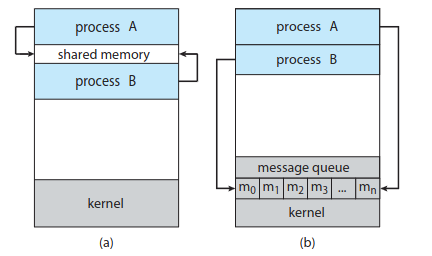
\includegraphics[width=0.8\linewidth]{figures/IPC.png}
    \caption{Hai cơ chế giao tiếp: a) Shared-Memory b) Message-Passing}
    \label{fig:ipc}
\end{figure}
\subsection{Pipe trong UNIX/xv6}

Pipe là một dạng IPC \textbf{unidirectional, half-duplex}, hiện thực dưới dạng
\textbf{bounded buffer} trong kernel -- minh họa kinh điển của
\textbf{producer-consumer problem} (Dijkstra, 1965).

\begin{figure}[H]
    \centering
    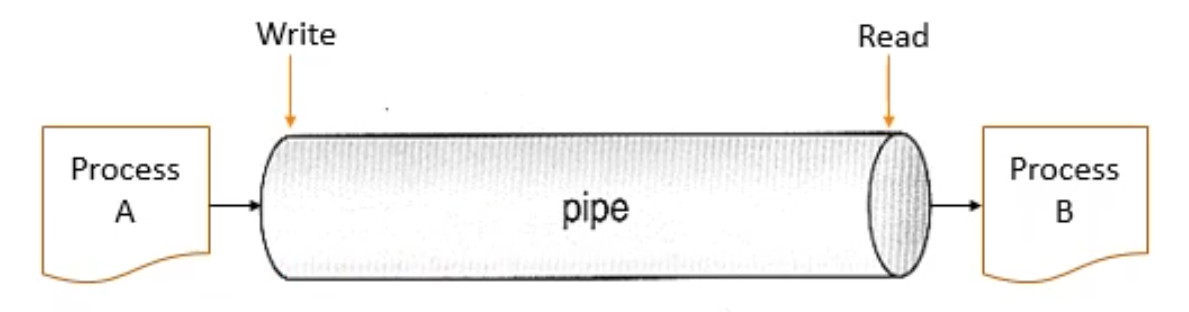
\includegraphics[width=0.8\linewidth]{figures/Pipe.png}
    \caption{Unix pipe}
    \label{fig:pipe}
\end{figure}

\begin{itemize}
    \item[+] Unidirectional: Dữ liệu chỉ được truyền theo một hướng.
    \item[+] Half-duplex: Tại một thời điểm, chỉ có một tiến trình được đọc hoặc ghi.
    \item[+] Bounded buffer: Pipe có kích thước cố định, khi đầy tiến trình ghi sẽ bị
    chặn, khi rỗng tiến trình đọc sẽ bị chặn.
\end{itemize}

\textbf{producer - consumer problem}, hay còn gọi là bài toán Bounded-Buffer (Bộ đệm có kích thước giới hạn), là một trong những bài toán kinh điển nhất trong khoa học máy tính về đồng bộ hóa đa tiến trình (multi-process synchronization). Nó được Edsger W. Dijkstra đưa ra vào năm 1965.
Hãy tưởng tượng một hệ thống có ba thành phần chính:
\begin{itemize}
    \item[]Producer (Người sản xuất): Một hoặc nhiều tiến trình (process/thread) liên tục tạo ra dữ liệu mới.
    \item[]Consumer (Người tiêu dùng): Một hoặc nhiều tiến trình liên tục lấy dữ liệu đó ra để xử lý.
    \item[]Buffer (Bộ đệm): Một vùng nhớ dùng chung (shared memory) có kích thước cố định ($N$ phần tử) để chứa dữ liệu do Producer tạo ra trước khi Consumer kịp lấy đi.
\end{itemize}

\begin{figure}[H]
    \centering
    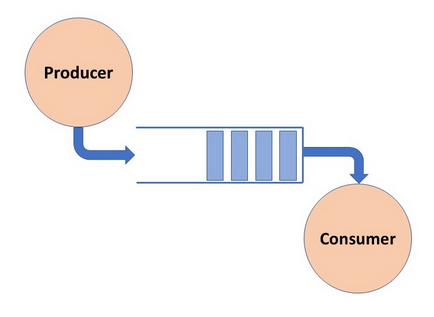
\includegraphics[width=0.8\linewidth]{figures/ProCon.png}
    \caption{Producer - Consumer Problem}
    \label{fig:ProCon}
\end{figure}

Bởi vì cả Producer và Consumer đều chạy song song (concurrently) và cùng thao tác trên một bộ đệm chung, các vấn đề nghiêm trọng sẽ xảy ra nếu không có cơ chế kiểm soát:
\begin{itemize}
    \item[]\textbf{Vượt quá giới hạn}: Producer không được phép thêm dữ liệu khi bộ đệm đã đầy (phải ngủ/chờ đến khi có chỗ trống).
    \item[]\textbf{Lấy dữ liệu rác}: Consumer không được phép lấy dữ liệu khi bộ đệm đang trống (phải ngủ/chờ đến khi có dữ liệu mới).
    \item[]\textbf{Race Condition}: Nếu Producer và Consumer (hoặc hai Producer) cùng ghi/đọc vào một vị trí trong bộ đệm tại cùng một chu kỳ máy, dữ liệu sẽ bị ghi đè, sai lệch hoặc hỏng hóc.
\end{itemize}
Trong xv6, vấn đề này được giải quyết bằng cách sử dụng một trường khóa là \textit{SPINLOCK}. \\
Trong UNIX, pipe giống như một file: ta có thể ghi dữ liệu vào nó và đọc dữ liệu từ nó.
Tuy nhiên, file được lưu trữ trên đĩa, còn dữ liệu trong pipe hoàn toàn nằm trên bộ nhớ.

\textbf{Cấu trúc pipe baseline (v1):}

\begin{lstlisting}[caption={struct pipe -- v1 baseline, PIPESIZE = 512 byte},
                   language=C, label={lst:pipe_v1}]
#define PIPESIZE 512

struct pipe {
    struct spinlock lock;  // bao ve tat ca cac truong
    char data[PIPESIZE];   // bo dem vong 512 bytes
    uint nread;            // vi tri doc trong bo dem
    uint nwrite;           // vi tri ghi trong bo dem
    int  readopen;         // tin hieu kich hoat doc
    int  writeopen;        // tin hieu kich hoat ghi
};
\end{lstlisting}

Giải thích các trường:
\begin{itemize}\tightlist
    \item \textbf{SPINLOCK:} bảo vệ tất cả các trường còn lại, ngăn chặn race condition.
    \item \textbf{nread, nwrite (uint):} chỉ số tích lũy -- pipe \textbf{đầy} khi
    \code{nwrite == nread + PIPESIZE}, \textbf{rỗng} khi \code{nread == nwrite}.
    Truy cập vào bộ đệm vòng bằng modulo: \code{data[nwrite \% PIPESIZE]}.
    \item \textbf{readopen, writeopen (int):} biến logic cho phép đọc/ghi.
    \item \textbf{data[] (512 byte):} bộ đệm vòng có kích thước PIPESIZE = 512.
\end{itemize}

\textbf{Lãng phí bộ nhớ trong v1:} Bất cứ khi nào cần tạo một pipe mới, kernel gọi
\code{kalloc()} phân bổ 1 trang (PAGESIZE = 4096~Byte). Các trường chiếm $\sim$0.5~KB,
trường trống còn lại là $\sim$3.5~KB -- không được sử dụng và lãng phí.

\subsection{Circular Buffer (Bộ đệm vòng)}

Pipe sử dụng bộ đệm vòng với cấu trúc như sau:

\begin{itemize}\tightlist
    \item Writer advances HEAD pointer (nwrite) sau khi ghi dữ liệu.
    \item Reader advances TAIL pointer (nread) sau khi đọc dữ liệu.
    \item Khi pointer đạt cuối mảng, nó ``vòng lại'' vị trí đầu (wrap-around).
    \item Buffer FULL khi \code{nwrite == nread + PIPESIZE}.
    \item Buffer EMPTY khi \code{nread == nwrite}.
\end{itemize}

\begin{figure}[H]
    \centering
    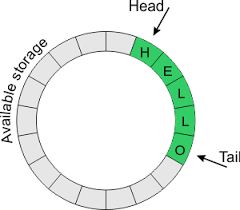
\includegraphics[width=0.7\textwidth]{figures/cirbuf.png}
    \caption{Circular Buffer}
    \label{fig:circular_buffer}
\end{figure}
\subsection{Cơ chế Spinlock và Sleep/Wakeup trong xv6}
Trước khi đến với vấn đề Producer - Consumer problem, thì ta đến với tiền thân của nó là Critical - Section problem. Cấu trúc của một tiến trình:
\begin{lstlisting}[language=C]
    while(true){
        entry section: // Yeu cau vao critical section
            critical section
        exit section: // Thong bao ket thuc critical section
            remainder section
    }
\end{lstlisting}
Trong hệ thống pipe của xv6, gồm 2 tiến trình $P_0$ và $P_1$, giả sử  $P_0$ là tiến trình ghi và $P_1$ là tiến trình đọc. Mỗĩ tiến trình có một 
phân đoạn mã, gọi là \textit{critical section}, nơi nó có thể truy cập và thay đổi các dữ liệu dùng chung với các tiến trình khác.Để giải quyết Critical - Section Problem, ta phải thiết kế với nguyên tắc là khi một tiến trình thực thi đoạn mã 
\textit{critical section} thì không có tiến trình khác có thể thực thi xen vào. Ba yêu cầu cần phải thỏa mãn:
\begin{itemize}
    \item \textbf{Mutual exclusion:} Nếu tiến trình $P_0$ đang thực thi critical section, thì tiến trình $P_1$ không được phép thực thi critical section.
    \item \textbf{Progress:} Nếu không có tiến trình nào trong critical section và một số tiến trình muốn vào, thì chỉ có những tiến trình đang không thực thi remainder section mới được quyết định tiến trình nào sẽ vào critical section tiếp theo, và quyết định này không được trì hoãn vô thời hạn.
    \item \textbf{Bounded waiting:} Tiến trình chờ trong critical section không được phép vượt quá một số hữu hạn các tiến trình khác đã vào critical section trước đó.
\end{itemize}
Trong chương trình đã học về Synchronization Tools trong môn hệ điều hành, để giải quyết Critical - Section Problem, ta có thể sử dụng: Peterson's Solution, các Hardware Instructions như test$\_$and$\_$set, compare$\_$and$\_$swap và các cơ chế như mutexlock, semaphore, monitor, ...\\
Trong hệ điều hành xv6, Synchronization Tools mà xv6 sử dụng là spin-lock (một phiên bản của mutex locks), có cấu trúc được định nghĩa trong file \textit{spinlock.h} như sau:
\begin{lstlisting}[language=C]
    #ifndef _SPINLOCK_H_
    #define _SPINLOCK_H_
    // Mutual exclusion lock.
    struct spinlock {
        uint locked;       // Is the lock held?

        // For debugging:
        char *name;        // Name of lock.
        struct cpu *cpu;   // The cpu holding the lock.
    };

    #endif
\end{lstlisting}
Tuy nhiên, do pipe phải trao đổi dữ liệu giữa hai tiến trình đọc và ghi, nên phải sử dụng thêm cơ chế sleep/wakeup để đồng bộ hóa hai tiến trình này. Đây là Producer - Consumer Problem, 
cơ chế sleep được định nghĩa trong file \textit{proc.h} như sau:
\begin{lstlisting}[language=C]
void sleep(void *chan, struct spinlock *lk)
{
  struct proc *p = myproc();
  
  // Must acquire p->lock in order to
  // change p->state and then call sched.
  // Once we hold p->lock, we can be
  // guaranteed that we won't miss any wakeup
  // (wakeup locks p->lock),
  // so it's okay to release lk.

  acquire(&p->lock);  //DOC: sleeplock1
  release(lk);

  // Go to sleep.
  p->chan = chan;
  p->state = SLEEPING;

  sched();

  // Tidy up.
  p->chan = 0;

  // Reacquire original lock.
  release(&p->lock);
  acquire(lk);
}
\end{lstlisting}
Và cơ chế wakeup được định nghĩa trong file \textit{proc.h} như sau:
\begin{lstlisting}[language=C]
// Wake up all processes sleeping on channel chan.
// Caller should hold the condition lock.
void wakeup(void *chan)
{
  struct proc *p;

  for(p = proc; p < &proc[NPROC]; p++) {
    if(p != myproc()){
      acquire(&p->lock);
      if(p->state == SLEEPING && p->chan == chan) {
        p->state = RUNNABLE;
      }
      release(&p->lock);
    }
  }
}
\end{lstlisting}
\subsection{Cách pipe hoạt động với tiến trình}

Giả sử có một tiến trình P. Một tiến trình có thể mở một số tệp tại bất kì thời điểm
nào. User code tham chiếu đến các tệp riêng lẻ bằng cách sử dụng một \textbf{bộ mô tả
tệp} (file descriptor) -- là một số nguyên 0, 1, 2,\ldots mà kernel dùng làm chỉ mục
(index) vào mảng \code{ofile[]} bên trong \code{struct proc}.

Trong cấu trúc của mỗi tiến trình, mảng \code{ofile[]} chứa các con trỏ đến các đối
tượng tệp (\code{struct file}). Mỗi đối tượng tệp có trường \code{type} -- ở đây mang
giá trị \code{FD\_PIPE} để chỉ ra đây là pipe -- và một con trỏ trỏ tới đối tượng
thực sự (\code{struct pipe}, inode, \ldots).

Trong trường hợp pipe, có 2 trường điều khiển truy cập: \code{readopen} và
\code{writeopen}. Mỗi trường chỉ bằng 1 khi còn ít nhất một file descriptor trỏ tới đầu
tương ứng của pipe.

\textbf{Quá trình tạo và sử dụng pipe (minh họa với P, R, W):}
\begin{enumerate}\tightlist
    \item Tiến trình P gọi \code{pipe(fd[])} -- kernel cấp phát \code{struct pipe},
    tạo 2 \code{struct file} (READABLE và WRITEABLE), tìm 2 ô trống trong
    \code{ofile[]} của P và trả về 2 file descriptor, ví dụ \textbf{fd=2} (read end)
    và \textbf{fd=4} (write end).

    \item P gọi \code{fork()} để tạo 2 tiến trình con \textbf{R} (đọc) và \textbf{W}
    (ghi). Do \code{fork()} sao chép toàn bộ \code{ofile[]}, cả R và W đều kế thừa
    hai file descriptor trên và cùng trỏ vào một \code{struct pipe} duy nhất trong
    kernel.

    \item Mỗi tiến trình đóng đầu mà nó không cần:
    \begin{itemize}\tightlist
        \item R gọi \code{close(fd=4)} $\Rightarrow$ \code{ofile[4] = NULL} (đóng write end).
        \item W gọi \code{close(fd=2)} $\Rightarrow$ \code{ofile[2] = NULL} (đóng read end).
    \end{itemize}

    \item W gửi dữ liệu đến R bằng cách gọi \code{write(fd=4, buf, n)}: kernel gọi
    \code{pipewrite()} để sao chép dữ liệu từ user space vào bộ đệm vòng của pipe
    trong kernel. Nếu bộ đệm đầy, W \code{sleep()} chờ R lấy bớt dữ liệu ra.

    \item R đọc dữ liệu bằng cách gọi \code{read(fd=2, buf, n)}: kernel gọi
    \code{piperead()} để sao chép dữ liệu từ bộ đệm vòng ra user space của R. Nếu
    bộ đệm rỗng, R \code{sleep()} chờ W ghi thêm.
\end{enumerate}

\subsection{Thông lượng IPC (IPC Throughput)}

Thông lượng của pipe được tính theo công thức:

\begin{equation}
\text{Throughput} = \frac{\text{DataTransfer (byte)}}{\text{TimeTransfer (giây)}}
= \frac{\text{total\_bytes} \times \text{TICKS\_PER\_SEC}}{\text{elapsed\_ticks}}
\end{equation}

Với:
\begin{itemize}
    \item \textbf{total\_bytes}: là tổng số byte dữ liệu cần truyền qua pipe.
    \item \textbf{TICKS\_PER\_SEC}: là số tick trong 1 giây, xv6 sử dụng timer interrupt để tăng giá trị của tick lên 1.
    \item \textbf{elapsed\_ticks}: là thời gian truyền hết dữ liệu qua pipe theo ticks.
\end{itemize}
Đơn vị đo chính: \textbf{Byte/s} (hoặc KB/s, MB/s).
Lưu ý: $1\,\text{MB/s} = 10^6\,\text{B/s}$ còn
$1\,\text{MiB/s} = 2^{20}\,\text{B/s} \approx 1.049 \times 10^6\,\text{B/s}$
-- hai đơn vị này khác nhau về cơ số.

% ===========================================================================
\section{Phân tích Baseline (v1)}
\label{sec:baseline}
% ===========================================================================


\subsection{Đường đi của một lần write/read qua pipe}

User process \textbf{không gọi trực tiếp} \code{pipewrite()}/\code{piperead()} mà gọi qua hàm \code{write()}/\code{read()} trong userspace và được định nghĩa trong file \textit{sysfile.c}.
Mỗi lần ghi/đọc trong đi qua một chuỗi các hàm trong kernel.

% ---- TikZ diagram: write/read path through pipe ----
\begin{figure}[H]
\centering
\begin{minipage}{0.46\textwidth}
\centering
\begin{tikzpicture}[
  unode/.style={rectangle, draw=black, fill=white,
                minimum width=5.6cm, minimum height=0.6cm,
                align=center, font=\small\ttfamily},
  knode/.style={rectangle, draw=black, fill=white,
                minimum width=5.6cm, minimum height=0.6cm,
                align=center, font=\small\ttfamily},
  arr/.style={-Stealth, thick}
]
\node[unode] (n0) at (0,  0.0) {write(fd, buf, n)};
\node[knode] (n1) at (0, -1.0) {uservec $\to$ usertrap};
\node[knode] (n2) at (0, -1.9) {syscall() $\to$ sys\_write()};
\node[knode] (n3) at (0, -2.8) {argfd() $\to$ filewrite()};
\node[knode] (n4) at (0, -3.7) {pipewrite()};
\node[knode] (n5) at (0, -4.6) {prepare\_return() $\to$ sret};
\node[unode] (n6) at (0, -5.6) {write() returns $n$};
\draw[arr] (n0)--(n1); \draw[arr] (n1)--(n2);
\draw[arr] (n2)--(n3); \draw[arr] (n3)--(n4);
\draw[arr] (n4)--(n5); \draw[arr] (n5)--(n6);
\draw[dashed] (-3.1,-0.38) rectangle (3.1,-5.05);
\end{tikzpicture}
\par\smallskip\small(a) Writer path
\end{minipage}
\hfill
\begin{minipage}{0.46\textwidth}
\centering
\begin{tikzpicture}[
  unode/.style={rectangle, draw=black, fill=white,
                minimum width=5.6cm, minimum height=0.6cm,
                align=center, font=\small\ttfamily},
  knode/.style={rectangle, draw=black, fill=white,
                minimum width=5.6cm, minimum height=0.6cm,
                align=center, font=\small\ttfamily},
  arr/.style={-Stealth, thick}
]
\node[unode] (n0) at (0,  0.0) {read(fd, buf, n)};
\node[knode] (n1) at (0, -1.0) {uservec $\to$ usertrap};
\node[knode] (n2) at (0, -1.9) {syscall() $\to$ sys\_read()};
\node[knode] (n3) at (0, -2.8) {argfd() $\to$ fileread()};
\node[knode] (n4) at (0, -3.7) {piperead()};
\node[knode] (n5) at (0, -4.6) {prepare\_return() $\to$ sret};
\node[unode] (n6) at (0, -5.6) {read() returns $n$};
\draw[arr] (n0)--(n1); \draw[arr] (n1)--(n2);
\draw[arr] (n2)--(n3); \draw[arr] (n3)--(n4);
\draw[arr] (n4)--(n5); \draw[arr] (n5)--(n6);
\draw[dashed] (-3.1,-0.38) rectangle (3.1,-5.05);
\end{tikzpicture}
\par\smallskip\small(b) Reader path
\end{minipage}
\caption{Đường đi \texttt{write()}/\texttt{read()} qua pipe trong xv6.
  Khung nét đứt = Kernel (Supervisor Mode); ô trắng = User space.}
\label{fig:pipe_path}
\end{figure}

\textbf{Phân tích chi tiết từng bước:}

\begin{table}[H]
\centering
\scriptsize
\setlength{\tabcolsep}{3pt}
\renewcommand{\arraystretch}{0.88}
\caption{Map từng hàm trong đường đi write/read pipe $\to$ file nguồn trong xv6}
\begin{tabularx}{\linewidth}{p{2.7cm}p{2.7cm}p{2.1cm}p{1.9cm}X}
\toprule
\textbf{Hàm (Write)} & \textbf{Hàm (Read)} & \textbf{File} & \textbf{Dòng} & \textbf{Mô tả} \\
\midrule
\code{ecall} & \code{ecall}
  & ISA (RISC-V) & -- & CPU trap sang supervisor mode; \code{pc} $\to$ \code{stvec}; lưu \code{pc} vào \code{sepc} \\
\code{uservec} & \code{uservec}
  & \code{trampoline.S} & :18 & Lưu 32 regs vào \code{trapframe}; đổi \code{satp} sang kernel page table; nhảy tới \code{usertrap()} \\
\code{usertrap()} & \code{usertrap()}
  & \code{trap.c} & :38 & Đọc \code{scause=8} (syscall), gọi \code{syscall()}; xử lý interrupt/exception \\
\code{syscall()} & \code{syscall()}
  & \code{syscall.c} & :132 & Đọc reg \code{a7} (SYS\_write=16 / SYS\_read=63), dispatch bảng \code{syscalls[]} \\
\code{sys\_write()} & \code{sys\_read()}
  & \code{sysfile.c} & :83 / :69 & \code{argfd()}, \code{argaddr()}, \code{argint()} đọc 3 args từ \code{a0,a1,a2} \\
\code{argfd()} & \code{argfd()}
  & \code{sysfile.c} & :22 & Validate \code{fd} $\in [0,\text{NOFILE})$; trả về \code{struct file*} từ \code{myproc()->ofile[fd]} \\
\code{filewrite()} & \code{fileread()}
  & \code{file.c} & :135 / :107 & Kiểm tra \code{f->type == FD\_PIPE}; dispatch $\to$ \code{pipewrite(f->pipe,...)} \\
\code{pipewrite()} & \code{piperead()}
  & \code{pipe.c} & :243 / :465 & \code{acquire(\&lock)}; vòng lặp: copyin/copyout từng byte, kiểm tra đầy/rỗng, sleep/wakeup \\
\code{copyin()} & \code{copyout()}
  & \code{vm.c} & :381 / :343 & \code{walkaddr()} dịch VA$\to$PA (Sv39 3-level), sau đó \code{memmove} copy dữ liệu \\
\code{walkaddr()} & \code{walkaddr()}
  & \code{vm.c} & :121 & Duyệt 3 cấp PTE (9+9+9+12 bit), kiểm tra bit V/U/R/W; trả về PA \\
\code{wakeup(\&nread)} & \code{wakeup(\&nwrite)}
  & \code{proc.c} & :742 & Quét \code{proc[NPROC]} (64 entry), đổi \code{SLEEPING$\to$RUNNABLE} nếu \code{chan} khớp \\
\code{prepare\_return()} & \code{prepare\_return()}
  & \code{trap.c} & :100 & Đặt \code{sstatus.SPP=0} (user mode), \code{sepc=epc}; set \code{stvec$\to$uservec} \\
\code{userret$\to$sret} & \code{userret$\to$sret}
  & \code{trampoline.S} & :101 & Khôi phục 32 regs; đổi \code{satp}$\to$user PT; \code{sret}: supervisor$\to$user \\
\bottomrule
\end{tabularx}
\renewcommand{\arraystretch}{1}
\end{table}

$\Rightarrow$ Throughput không chỉ phụ thuộc vào \code{kernel/pipe.c}, mà còn phụ thuộc vào rất nhiều yếu tố khác: trap, syscall dispatch, file layer, copy memory, page table walk,
TLB, cache, spinlock, sleep/wakeup, scheduler.

% ---------------------------------------------------------------------------
%\subsubsection{Chứng minh thực nghiệm: kernel trace đường đi}
%\label{sssec:pipe_trace}

%Để \textbf{chứng minh thực nghiệm} rằng đường đi trong Hình~\ref{fig:pipe_path} là
%đúng, chúng tôi thêm \code{printf} vào 5 kernel file, kiểm soát bởi flag
%\code{-DPIPE\_TRACE=1} ở compile time.

%\begin{table}[H]
%\centering\footnotesize
%\caption{Các điểm kernel trace được thêm để chứng minh đường đi}
%\label{tab:pipe_trace_files}
%\begin{tabularx}{\linewidth}{clllX}
%\toprule
%\textbf{Step} & \textbf{File} & \textbf{Hàm} & \textbf{Điều kiện lọc} & \textbf{Nội dung in ra} \\
%\midrule
%{[W/R 1]} & \code{trap.c}     & \code{usertrap()}         & scause=8, pid=ptdemo, FD\_PIPE & scause, pid, epc, syscall\# \\
%{[W/R 2]} & \code{syscall.c}  & \code{syscall()}          & SYS\_write/read + FD\_PIPE     & tên syscall, num, pid \\
%{[W/R 3,4]} & \code{sysfile.c} & \code{sys\_write/read()}, \code{argfd()} & FD\_PIPE & fd, addr, n; file* type \\
%{[W/R 5]} & \code{file.c}     & \code{filewrite/read()}   & \code{f->type == FD\_PIPE}     & n, dispatch tới pipe \\
%{[W/R 6]} & \code{pipe.c}     & \code{pipewrite/read()}   & luôn (v1)                     & enter/exit, số lần copyin/copyout \\
%{[W/R 7]} & \code{trap.c}     & \code{prepare\_return()}  & \code{pipe\_trace\_active} flag & sstatus.SPP, sepc, stvec \\
%\bottomrule
%\end{tabularx}
%\end{table}

%\textbf{Cách build và chạy:}
%\begin{lstlisting}[language=bash]
%make clean
%make PIPE_VERSION=1 PIPE_TRACE=1   # build kernel + userland voi trace
%make PIPE_VERSION=1 PIPE_TRACE=1 qemu
%# Trong QEMU gõ: ptdemo
%\end{lstlisting}

% \textbf{Output thực tế từ terminal QEMU} khi chạy \code{ptdemo}:
%\begin{lstlisting}[language={}, basicstyle=\tiny\ttfamily, frame=single,
%    backgroundcolor=\color{gray!8},
%    caption={Output kernel trace xac nhan dung duong di write/read v1},
%    label={lst:pipe_trace_out}]
%$ ptdemo
%>>> BUOC 1: write(fd[1], "HELLO", 5)
%    [user] ecall -> kernel...
%[TRACE W1] usertrap()    : scause=8 (ecall) pid=3 epc=0x3ca syscall#=16 (write)
%[TRACE W2] syscall()     : SYS_write (num=16) pid=3 -> dispatch
%[TRACE W3] sys_write()   : fd=4  addr=0x3fa8  n=5
%[TRACE W4] argfd()       : fd=4 -> file* type=FD_PIPE -> filewrite()
%[TRACE W5] filewrite()   : FD_PIPE n=5 -> pipewrite()
%[TRACE W6] pipewrite()   : enter n=5  nwrite=0  nread=0
%[TRACE   ]   copyin()    : 5 call(s) x 1B, user[0x3fa8+0..4] -> data[]
%[TRACE   ]   wakeup()    : &pi->nread (unconditional, reader may not be sleeping)
%[TRACE W6] pipewrite()   : exit  wrote=5  nwrite=5
%[TRACE W7] prepare_return: sstatus.SPP<-0  sepc<-0x3ce  stvec<-trampoline
%[TRACE   ]                 sret -> user mode
%    [user] write() tra ve 5
%
%>>> BUOC 2: read(fd[0], buf, 5)
%    [user] ecall -> kernel...
%[TRACE R1] usertrap()    : scause=8 (ecall) pid=3 epc=0x3c2 syscall#=5 (read)
%[TRACE R2] syscall()     : SYS_read (num=5) pid=3 -> dispatch
%[TRACE R3] sys_read()    : fd=3  addr=0x3fb0  n=5
%[TRACE R4] argfd()       : fd=3 -> file* type=FD_PIPE -> fileread()
%[TRACE R5] fileread()    : FD_PIPE n=5 -> piperead()
%[TRACE R6] piperead()    : enter n=5  nwrite=5  nread=0
%[TRACE   ]   copyout()   : 5 call(s) x 1B, data[] -> user[0x3fb0+0..4]
%[TRACE   ]   wakeup()    : &pi->nwrite
%[TRACE R6] piperead()    : exit  read=5  nread=5
%[TRACE R7] prepare_return: sstatus.SPP<-0  sepc<-0x3c6  stvec<-trampoline
%[TRACE   ]                 sret -> user mode
%    [user] read() tra ve 5, nhan duoc: "HELLO"
%\end{lstlisting}

%\begin{figure}[H]
%\centering
%\includegraphics[width=\linewidth]{ptdemo_trace.png}
%\caption{Ảnh chụp terminal QEMU khi chạy \texttt{ptdemo} -- kernel trace xác nhận đường đi write/read qua pipe v1.}
%\label{fig:ptdemo_trace}
%\end{figure}

%\textbf{Đối chiếu trace $\leftrightarrow$ sơ đồ (Hình~\ref{fig:pipe_path}):}
%\begin{itemize}\tightlist
%  \item \code{[W1]}: \code{scause=8} xác nhận đây là syscall trap (ecall từ user space)
%  \item \code{[W2]}: \code{SYS\_write=16} -- dispatch đúng entry trong bảng \code{syscalls[]}
%  \item \code{[W3,W4]}: \code{fd=4} là write-end của pipe; \code{argfd()} trả về \code{FD\_PIPE}
%  \item \code{[W5]}: \code{filewrite()} phân nhánh đúng vào \code{FD\_PIPE}, không đi vào \code{FD\_INODE} hay \code{FD\_DEVICE}
%  \item \code{[W6]}: \code{pipewrite()} gọi \code{copyin()} đúng \textbf{5 lần} (HELLO = 5 byte) -- chứng minh v1 là byte-by-byte
%  \item \code{[W6]}: \code{wakeup(\&pi->nread)} vô điều kiện dù reader chưa chắc đang ngủ -- bottleneck \#2
%  \item \code{[W7]}: \code{prepare\_return()} đặt \code{sstatus.SPP=0} (supervisor→user) trước \code{sret}
%  \item Read path \code{[R1--R7]}: đối xứng hoàn toàn; \code{copyout()} thay \code{copyin()}; \code{nwrite=5} khi reader vào (dữ liệu đã có sẵn)
%\end{itemize}

% ---------------------------------------------------------------------------
\subsection{Source code đầy đủ -- pipealloc, pipewrite và piperead v1}
\label{ssec:v1src}
% ---------------------------------------------------------------------------

Source code sau đây là \textbf{bản gốc xv6} tại \code{PIPE\_VERSION == 1},
trích trực tiếp từ \code{kernel/pipe.c}.
Đây là điểm xuất phát của toàn bộ chuỗi tối ưu.

% ------- pipealloc -------
\subsubsection{struct pipe và pipealloc() v1}

\textbf{Cấu trúc dữ liệu \code{struct pipe} v1} (kernel/pipe.c:43):

\begin{lstlisting}[caption={struct pipe v1 -- buffer nhúng 512 byte (kernel/pipe.c:43)},
                   language=C, label={lst:pipe_struct_v1}]
#define PIPESIZE 512

struct pipe {
  struct spinlock lock;   /* bao ve toan bo struct */
  char data[PIPESIZE];    /* circular buffer 512 byte*/
  uint nread;             /* so byte da doc  */
  uint nwrite;            /* so byte da ghi  */
  int  readopen;          /* 1 neu read-end con mo */
  int  writeopen;         /* 1 neu write-end con mo */
};
\end{lstlisting}


\medskip
\textbf{pipealloc()} được gọi từ \code{sys\_pipe()} khi user gọi syscall \code{pipe(int[2])}:

\begin{lstlisting}[caption={pipealloc() -- v1, khoi tao pipe (kernel/pipe.c:151)},
                   language=C, label={lst:pipealloc_v1}]
int
pipealloc(struct file **f0, struct file **f1)
{
  // Khoi tao mot cau truc pipe *pi
  struct pipe *pi;

  // Khoi tao gia tri ban dau cho pipe la trong
  pi = 0;
  // Con tro tro toi cac file duoc gan ban dau la 0 de khong tro den file nao
  *f0 = *f1 = 0;
  // Ham filealloc() (nam trong kernel/file.c) tra ve con tro file neu thanh cong,
  // tra ve 0 neu that bai. Neu mot trong hai file that bai, di den nhan bad
  if((*f0 = filealloc()) == 0 || (*f1 = filealloc()) == 0)
    goto bad;
  // Ham kalloc() (nam trong kernel/kalloc.c): cap phat mot page 4096 bytes,
  // tra ve con tro neu thanh cong, tra ve 0 neu that bai.
  // Neu cap phat khong thanh cong, di den nhan bad
  if((pi = (struct pipe*)kalloc()) == 0)
    goto bad;
  // Cap phat thanh cong: gan cac truong readopen, writeopen = 1 (ca hai dau deu mo),
  // vi tri ghi == vi tri doc == 0 (buffer rong)
  pi->readopen  = 1;
  pi->writeopen = 1;
  pi->nwrite    = 0;
  pi->nread     = 0;
  // Khoi tao khoa lien ket voi pipe bang ham initlock()
  initlock(&pi->lock, "pipe");
  // Gan gia tri cho cac file doc va ghi.
  // Mot struct file (trong file.c) gom: type (FD_NONE/FD_PIPE/FD_INODE),
  // ref, readable, writable, struct pipe*, struct inode*, off
  (*f0)->type = FD_PIPE;  // f0: read-end
  (*f0)->readable = 1;
  (*f0)->writable = 0;
  (*f0)->pipe = pi;
  (*f1)->type = FD_PIPE;  // f1: write-end
  (*f1)->readable = 0;
  (*f1)->writable = 1;
  (*f1)->pipe = pi;
  return 0;

 bad:
  // Nhan bad: giai phong trang bang kfree(), dong cac file bang fileclose()
  if(pi)  kfree((char*)pi);
  if(*f0) fileclose(*f0);
  if(*f1) fileclose(*f1);
  return -1;
}
\end{lstlisting}

\textbf{Nhận xét pipealloc() v1 -- 2 điểm đáng chú ý:}
\begin{enumerate}\tightlist
  \item \textbf{kalloc() lãng phí:} \code{kalloc()} cấp phát đúng \textbf{1 trang = 4096 byte}.
  Nhưng \code{struct pipe} v1 chỉ chiếm $\approx 560$ byte
  (spinlock $\approx 40$B $+$ data[512] $+$ 4×uint $+$ 2×int).
  Phần còn lại $\approx 3{,}536$ byte trong trang bị \textbf{lãng phí hoàn toàn}.

\end{enumerate}

\subsubsection{pipewrite() và piperead() v1}

\begin{lstlisting}[caption={pipewrite() -- v1 baseline, byte-by-byte (kernel/pipe.c:243)},
                   language=C, label={lst:pipewrite_v1}]
int
pipewrite(struct pipe *pi, uint64 addr, int n)
{
  int i = 0;
  struct proc *pr = myproc();

  // Lay khoa truoc khi vao vung critical section
  acquire(&pi->lock);
  // Ghi tung byte du lieu vao bo dem
  while(i < n){
    // Neu read-end da dong hoac tien trinh bi ket lieu, ghi that bai
    if(pi->readopen == 0 || killed(pr)){
      release(&pi->lock);
      return -1;
    }
    // Bo dem day (nwrite - nread == PIPESIZE): danh thuc reader dang cho,
    // sau do tien trinh ghi chuyen sang che do ngu cho den khi co cho trong
    if(pi->nwrite == pi->nread + PIPESIZE){
      wakeup(&pi->nread);
      sleep(&pi->nwrite, &pi->lock);
    } else {
      char ch;
      // Doc 1 byte tu user address space vao bien tam trong kernel
      if(copyin(pr->pagetable, &ch, addr + i, 1) == -1)
        break;
      // Ghi byte vao vi tri hien tai trong bo dem vong, tang nwrite
      pi->data[pi->nwrite++ % PIPESIZE] = ch;
      i++;
    }
  }
  // Ghi xong: danh thuc tien trinh doc de doc tiep, tra lai khoa
  wakeup(&pi->nread);
  release(&pi->lock);
  return i;
}
\end{lstlisting}

\begin{lstlisting}[caption={piperead() -- v1 baseline, byte-by-byte (kernel/pipe.c:465)},
                   language=C, label={lst:piperead_v1}]
int
piperead(struct pipe *pi, uint64 addr, int n)
{
  int i;
  struct proc *pr = myproc();
  char ch;

  // Lay khoa truoc khi vao vung critical section
  acquire(&pi->lock);
  // Kiem tra xem pipe co rong va write-end con mo hay khong.
  // Neu rong va writer van con, chuyen sang che do ngu cho den khi co du lieu
  while(pi->nread == pi->nwrite && pi->writeopen){
    // Kiem tra tien trinh co bi ket lieu hay chua, neu bi ket lieu tra ve -1
    if(killed(pr)){
      release(&pi->lock);
      return -1;
    }
    // Bo dem rong: chuyen sang che do ngu, giai phong khoa cho writer ghi
    sleep(&pi->nread, &pi->lock);
  }
  // Doc tung byte du lieu tu bo dem
  for(i = 0; i < n; i++){
    // Da doc het du lieu trong bo dem, dung
    if(pi->nread == pi->nwrite)
      break;
    // Doc byte tai vi tri hien tai trong bo dem vong, tang nread
    ch = pi->data[pi->nread++ % PIPESIZE];
    // Ghi 1 byte tu bien tam trong kernel ra user address space
    if(copyout(pr->pagetable, addr + i, &ch, 1) == -1)
      break;
  }
  // Doc xong: danh thuc tien trinh ghi dang cho, tra lai khoa
  wakeup(&pi->nwrite);
  release(&pi->lock);
  return i;
}
\end{lstlisting}

% ------- pipeclose -------
\subsubsection{pipeclose() v1}

\textbf{pipeclose()} được gọi khi tiến trình đóng một đầu pipe (qua syscall
\code{close()}). Hàm nhận tham số \code{writable} để phân biệt đóng write-end
(\code{writable=1}) hay read-end (\code{writable=0}), đặt cờ tương ứng về 0,
đánh thức bên đối diện nếu đang ngủ, và giải phóng trang vật lý khi cả hai đầu
đều đã đóng:

\begin{lstlisting}[caption={pipeclose() -- v1, dong mot dau pipe (kernel/pipe.c:201)},
                   language=C, label={lst:pipeclose_v1}]
void
pipeclose(struct pipe *pi, int writable)
{
  // writable=1: dong write-end; writable=0: dong read-end
  // Lay khoa cho doi tuong pipe
  acquire(&pi->lock);
  // Dong viec ghi: dat writeopen = 0
  if(writable){
    pi->writeopen = 0;
    // Danh thuc bat ki tien trinh doc nao dang cho, bao hieu write-end da dong
    wakeup(&pi->nread);
  // Dong viec doc: dat readopen = 0
  } else {
    pi->readopen = 0;
    // Danh thuc bat ky tien trinh ghi nao dang cho, bao hieu read-end da dong
    wakeup(&pi->nwrite);
  }
  // Neu ca hai dau da dong -> hoan thanh: tra lai khoa va giai phong trang bo nho.
  // Neu chua thi chi tra lai khoa, giu nguyen pipe cho dau kia tiep tuc dung
  if(pi->readopen == 0 && pi->writeopen == 0){
    release(&pi->lock);
    kfree((char*)pi);
  } else
    release(&pi->lock);
}
\end{lstlisting}

\textbf{Nhận xét source code v1 -- 3 vấn đề chính:}
\begin{enumerate}\tightlist
  \item \textbf{byte-by-byte copy:} Mỗi byte = 1 lần \code{copyin}/\code{copyout}
  = 1 lần \code{walkaddr()}. Với 4096~byte,
  cần 4096 lần gọi \code{walkaddr()} do đó chi phí gọi syscall là rất cao.

  \item \textbf{wakeup vô điều kiện:} Dòng cuối \code{pipewrite} gọi
  \code{wakeup(\&pi->nread)} dù reader có thể \emph{không ngủ} -- quét 64 entry
  \code{proc[]} lãng phí thời gian quét mỗi lần ghi.

  \item \textbf{PIPESIZE = 512:} Buffer chỉ 512~byte. Một lần ghi chunk-bytes = 4096 bị
  chia 8 đợt, mỗi đợt khi buffer đầy writer phải \code{sleep}/\code{wakeup} để làm rỗng
  bộ đệm, dẫn đến giảm băng thông.
\end{enumerate}
% ---------------------------------------------------------------------------
Từ các phân tích ở các mục trên, các yếu tố tác động đến băng thông là:

\begin{enumerate}
    \item \textbf{Chi phí gọi syscall}.
    \item \textbf{Kích thước pipe buffer:} 512 bytes quá bé, cần tăng kích thước bộ đệm.
    \item \textbf{copyin/copyout:} cần có cách để copy một lúc nhiều bytes chứ không phải 1 byte.
    \item \textbf{Spinlock \& sleep/wakeup:} Cần có cơ chế synchonization tốt hơn.
\end{enumerate}
Ngoài ra, còn một số yếu tố khác cũng ảnh hưởng đến băng thông:
\begin{enumerate}
    \item \textbf{Scheduler:} xv6 sử dụng cơ chế lập lịch Round-Robin, có cơ chế lập lịch nào tốt hơn không?  
    \item \textbf{CPU cache:} Hầu hết các dòng CPU hiện đại(Intel, AMD, ARM) đều có cacheline là 64 bytes, nếu các dữ liệu của writer và reader nằm trong cùng một cacheline thì sẽ xảy ra false sharing.
\end{enumerate}


Tổng hợp các kiến thức trên, một lần truyền $n$ byte qua pipe trong v1 tốn:

\begin{verbatim}
T_v1(n) = T_syscall_write
        + n * T_copyin(1)          (mỗi byte 1 lần copyin)
        + n * T_lock_acquire_release
        + n * T_check
        + ceil(n/PIPESIZE) * T_sleep_wakeup
        + (đợi xung cho reader)
\end{verbatim}

%\begin{table}[H]
%\centering
%\caption{Phân rã chi phí v1 tại \code{chunk\_bytes = 4096} (ước lượng cycle)}
%\begin{tabular}{lrr}
%\toprule
%\textbf{Hợp phần} & \textbf{Cycle ước tính} & \textbf{Phần \%} \\
%\midrule
%$4096\times$ copyin(1) -- fixed overhead $\approx 80$~c & $\sim 327{,}680$ & $\sim 74\%$ \\
%$4096\times$ lock acquire+release $\approx 20$~c & $\sim 81{,}920$ & $\sim 9\%$ \\
%$7\times$ sleep/wakeup $\approx 2000$~c & $\sim 14{,}000$ & $\sim 2\%$ \\
%$4096\times$ check + branch & $\sim 20{,}000$ & $\sim 2\%$ \\
%$1\times$ T\_syscall\_write & $\sim 400$ & $\sim 0.1\%$ \\
%Scheduler delay ($\sim 10$~ms tick) & -- & $\sim 13\%$ \\
%\midrule
%\textbf{Tổng cộng (writer + reader)} & $\boldsymbol{\sim 888{,}000}$ & $100\%$ \\
%\bottomrule
%\end{tabular}
%\end{table}

\textbf{Nhận xét về \texttt{chunk\_bytes}:}
\texttt{chunk\_bytes} càng lớn thì số lần gọi syscall càng ít, giúp giảm
overhead trap vào kernel. Tuy nhiên, chunk lớn hơn đồng nghĩa mỗi lần
\code{write()} phải chờ reader drain buffer nhiều lần hơn, làm tăng chi phí
\code{sleep()}/\code{wakeup()} trên mỗi lần gọi -- đây là sự đánh đổi giữa
ít syscall và nhiều lần chờ đồng bộ. Do đó trong bài báo cáo này, chúng tôi sẽ đo băng thông từng version với các \code{chunk\_bytes} là 64, 128, 256, 512, 1024, 2048 và 4096 để xem băng thông thay đổi như nào.

\subsection{Các phiên bản tối ưu thông lượng}
Sau khi đã phân tích các yếu tố ảnh hưởng đến băng thông, chúng tôi đề xuất các phiên bản tối ưu thông lượng dựa trên các báo cáo tìm hiểu hàng tuần:
\begin{table}[H]
\centering
\caption{Các phiên bản tối ưu thông lượng}
\begin{tabular}{cl}
\toprule
\textbf{\#} & \textbf{Phiên bản tối ưu} \\
\midrule
1 & \vv{v2} -- Bulk Copy \\
2 & \vv{v3} -- Ring of Buffers \\
3 & \vv{v4} -- Multi-page \\
4 & \vv{v5} -- Lazy Wakeup \\
5 & \vv{v6} -- Priority Boost \\
6 & \vv{v7} -- Cache-line Align \\
7 & \vv{v8} -- All Combined \\
\bottomrule
\end{tabular}
\end{table}

\subsection{Đo băng thông của phiên bản v1}
Để đo được băng thông của phiên bản v1, chúng tôi đã viết ra chương trình C tại thư mục \textit{user/pipebench.c}, chương trình này sẽ đo băng thông của pipe bằng cách tạo ra 2 tiến trình, tiến trình cha (parent) ghi và tiến trình con (child) đọc. 
Dữ liệu tổng truyền đi mặc định có độ lớn là 4MiB bytes. Với \code{chunk\_bytes} là kích thước mỗi lần write()/read(). Để chạy chương trình này:
\begin{lstlisting}[language=bash]
    make clean
    make PIPE_VERSION=1 qemu
    # Sau khi QEMU chay, trong xv6:
    pipebench                     # quet chunk_bytes, total mac dinh ~4 MB
    pipebench chunk [total_bytes] # quet chunk, co dinh total
    pipebench total [chunk_bytes] # quet total, co dinh chunk
    # Vi du:
    pipebench chunk 1048576       # quet chunk voi total = 1 MB
    pipebench total 256           # quet total voi chunk = 256 B
\end{lstlisting}

Sau khi chạy xong, chúng tôi sẽ thu được kết quả trong file \textit{ipctp.txt} trong filesystem xv6. Để xem kết quả, chúng tôi có thể dùng lệnh \code{cat ipctp.txt} trong xv6.

\begin{table}[H]
\centering
\caption{Throughput baseline v1 (B/s) theo chunk\_bytes}
\begin{tabular}{rr}
\toprule
\textbf{chunk\_bytes} & \textbf{v1 (B/s)} \\
\midrule
64   & 198,782 \\
128  & 310,689 \\
256  & 419,430 \\
512  & 511,500 \\
1024 & 511,500 \\
2048 & 559,240 \\
4096 & 559,240 \\
\bottomrule
\end{tabular}
\end{table}


% ===========================================================================
\section{Các phiên bản tối ưu (v2--v8)}
\label{sec:versions}
% ===========================================================================

\subsection{v2 -- Bulk Copy}

Thay vì mỗi lần gọi copyin()/copyout() ta chỉ ghi/đọc được 1 byte, ta có thế ghi/đọc 1 khỗi \code{chunk\_bytes}
với mỗi lần copyin()/copyout() do đó chi phí $T_{v2}(n)$ sẽ giảm đi, thay vì là $n \cdot T_{\text{copyin}}(1)$ sẽ là $\lceil n/\text{chunk\_bytes} \rceil \cdot T_{\text{copyin}}(\text{chunk\_bytes})$.
Giải pháp này được gọi là Bulk Copy.
\begin{lstlisting}[caption={v2 -- pipewrite thay byte-by-byte bằng bulk copyin}, language=C]
// v2 - pipewrite:
int
pipewrite(struct pipe *pi, uint64 addr, int n)
{
  int i = 0;
  struct proc *pr = myproc();

  acquire(&pi->lock);
  while(i < n){
    if(pi->readopen == 0 || killed(pr)){
      release(&pi->lock);
      return -1;
    }
    if(pi->nwrite == pi->nread + PIPESIZE){
      wakeup(&pi->nread);
      sleep(&pi->nwrite, &pi->lock);
    } else {
      uint free_slots = PIPESIZE - (pi->nwrite - pi->nread);
      uint head_slot  = pi->nwrite % PIPESIZE;
      uint till_wrap  = PIPESIZE - head_slot;
      int to_copy = (int)umin((uint)(n - i), umin(free_slots, till_wrap));
      if(copyin(pr->pagetable, &pi->data[head_slot], addr + i, to_copy) == -1)
        break;
      pi->nwrite += to_copy;
      i          += to_copy;
    }
  }
  wakeup(&pi->nread);
  release(&pi->lock);
  return i;
}
\end{lstlisting}

\begin{lstlisting}[caption={v2 -- piperead thay byte-by-byte bằng bulk copyout}, language=C]
// v2 - piperead:
int
piperead(struct pipe *pi, uint64 addr, int n)
{
  int i = 0;
  struct proc *pr = myproc();

  acquire(&pi->lock);
  while(pi->nread == pi->nwrite && pi->writeopen){
    if(killed(pr)){
      release(&pi->lock);
      return -1;
    }
    sleep(&pi->nread, &pi->lock);
  }
  while(i < n){
    if(pi->nread == pi->nwrite)
      break;
    uint avail     = pi->nwrite - pi->nread;
    uint tail_slot = pi->nread % PIPESIZE;
    uint till_wrap = PIPESIZE - tail_slot;
    int to_copy = (int)umin((uint)(n - i), umin(avail, till_wrap));
    if(copyout(pr->pagetable, addr + i, &pi->data[tail_slot], to_copy) == -1){
      if(i == 0) i = -1;
      break;
    }
    pi->nread += to_copy;
    i         += to_copy;
  }
  wakeup(&pi->nwrite);
  release(&pi->lock);
  return i;
}
\end{lstlisting}
Hàm \code{umin(a, b)} trả về giá trị nhỏ hơn trong hai số nguyên không dấu.
Tại vòng lặp \code{while()} sẽ ghi 1 khối n = \code{chunk\_bytes} với các bước sau:
\begin{enumerate}
    \item Kiểm tra xem buffer đã đầy chưa, điều kiện \code{pi->nwrite == pi->nread + PIPESIZE} sẽ được kiểm tra ở mỗi lần ghi. Nếu buffer đã đầy thì sẽ đánh thức reader và sleep writer.
    \item Nếu chưa đầy thì tính toán số bytes còn trống trong buffer, vị trí con trỏ head bằng phép modulo vì nwrite có thể lớn hơn giá trị buffer hiện tại.
    \item Tính toán till$\_$wrap bytes có thể ghi trong 1 lần tính từ head đến cuối bộ đệm.
    \item So sánh số bytes có thể ghi vào, lấy giá trị nhỏ nhất bằng hàm \code{umin()}. Có 3 trường hợp có thể xảy ra:
    \begin{enumerate}
        \item Số bytes còn lại cần ghi là nhỏ nhất: \code{to\_copy = n - i}.
        \item Số bytes còn trống trong buffer lớn hơn số byte có thể ghi trong 1 lần,  xảy ra khi dữ liều đã được đọc trong piperead: \code{to\_copy = till\_wrap}.
        \item Số bytes còn trống trong buffer nhỏ hơn số bytes có thể  ghi trong 1 lần, xảy ra khi vẫn còn dữ liệu cũ chưa được đọc: \code{to\_copy = free\_slots}.
    \end{enumerate}
    \item Gọi copyin() để ghi khối dữ liệu vào buffer.
    \item Cập nhật con trỏ nwrite và i.
\end{enumerate}
Tại vòng lặp \code{while()} sẽ đọc 1 khối n = \code{chunk\_bytes} với các bước sau:
\begin{enumerate}
    \item Kiểm tra xem buffer đã rỗng chưa, điều kiện \code{pi->nread == pi->nwrite} sẽ được kiểm tra ở mỗi lần đọc. Nếu buffer đã rỗng thì sẽ sleep reader.
    \item Nếu chưa rỗng thì tính toán số bytes có thể đọc trong 1 lần tính từ tail đến cuối bộ đệm.
    \item So sánh số bytes có thể đọc vào, lấy giá trị nhỏ nhất bằng hàm \code{umin()}. Có 3 trường hợp có thể xảy ra:
    \begin{enumerate}
        \item Số bytes còn lại cần đọc là nhỏ nhất: \code{to\_copy = n - i}.
        \item Số bytes còn trống trong buffer lớn hơn số byte có thể đọc trong 1 lần,  xảy ra khi dữ liều đã được ghi trong pipewrite: \code{to\_copy = till\_wrap}.
        \item Số bytes còn trống trong buffer nhỏ hơn số bytes có thể đọc trong 1 lần, xảy ra khi vẫn còn dữ liệu cũ chưa được ghi: \code{to\_copy = avail}.
    \end{enumerate}
    \item Gọi copyout() để đọc khối dữ liệu từ buffer.
    \item Cập nhật con trỏ nread và i.
\end{enumerate}
\textbf{Ưu điểm:}
\begin{itemize}\tightlist
    \item Giảm số lần gọi copyin()/copyout() từ $n$ xuống $\lceil n/\text{chunk\_bytes} \rceil$.
    \item Không thay đổi cấu trúc dữ liệụ.
\end{itemize}

\textbf{Nhược điểm:}
\begin{itemize}\tightlist
    \item Vẫn bị giới hạn bởi PIPESIZE = 512~byte.
    \item Vẫn còn wrap-around: một lần ghi có thể bị cắt thành 2 lần copyin ở biên
    vòng tròn 512~byte.
    \item Critical section dài hơn (giữ spinlock trong khi copyin()/copyout() cả khối).
\end{itemize}

\subsubsection{Kết quả đo đạc v2}
Tương tự với v1, để đo băng thông của v2, ta cũng chạy như sau:
\begin{lstlisting}[language=bash]
    make clean
    make PIPE_VERSION=2 qemu // Ung voi v2
    \\ Sau khi QEMU chạy, trong xv6, chạy lệnh:
    pipebench
\end{lstlisting}
So sánh băng thông của v1 và v2:
\begin{table}[H]
\centering
\caption{So sánh throughput v1 vs v2 (B/s)}
\begin{tabular}{rrrr}
\toprule
\textbf{chunk\_bytes} & \textbf{v1 (B/s)} & \textbf{v2 (B/s)} & \textbf{Tăng} \\
\midrule
64   & 198,782 & 268,865   & $1.35\times$ \\
128  & 310,689 & 499,321   & $1.61\times$ \\
256  & 419,430 & 855,980   & $2.04\times$ \\
512  & 511,500 & 1,398,101 & $2.73\times$ \\
1024 & 511,500 & 1,613,193 & $3.15\times$ \\
2048 & 559,240 & 1,747,626 & $3.13\times$ \\
4096 & 559,240 & 1,823,610 & $3.26\times$ \\
\bottomrule
\end{tabular}
\end{table}
Ta thấy sự tăng trưởng giưa v1 và v2 là khá lớn, đặc biệt là ở \code{chunk\_bytes} lớn, lý do như sau:
\begin{itemize}
    \item Với \code{chunk\_bytes} nhỏ, số lần gọi syscall sẽ nhiều (số lần gọi syscall = \code{total\_bytes} / \code{chunk\_bytes}), do đó băng thông bị giới hạn bởi thời gian xử lý syscall.
    \item Với \code{chunk\_bytes} lớn, số lần gọi syscall đã giảm đi, do đó băng thông giờ theo chi phí số lần copyin()/copyout().
\end{itemize}
%\begin{figure}[H]
%\centering
%\includegraphics[width=0.92\textwidth]{bench_v1_v2.png}
%\caption{Kết quả chạy thực tế \code{pipebench} v1 vs v2 trong xv6/QEMU.
%Màu vàng = tăng $\geq 2\times$, màu xanh = tăng $\geq 1.5\times$.}
%\label{fig:bench_v1_v2_run}
%\end{figure}
\subsection{v3 -- Ring of Buffers}
Tuy nhiên v2 vẫn bị giới hạn bởi 512 bytes, do đó, khi gọi một chunk$\_$bytes lớn hơn so với bộ đệm thì bộ đệm sẽ 
thưởng xuyên bị đầy, và do đó cần gọi nhiều lần sleep()/wakeup(). Do đó, ta cần tăng dung lượng bộ đệm lên. \\
Một lý do nữa là khi ta cập một trang cho pipe thì có tận 3.5K bytes không được sử dụng dẫn đến bị lãng phí dữ liệu không được sử dụng đó.
Để tăng dụng lượng bộ đệm ta thay đổi trường data[] trong trường pipe như sau, giả sử tăng lên 2048 bytes:

\begin{lstlisting}[language=C]
#define PIPESIZE 2048

struct pipe {
  struct spinlock lock;   /* bao ve toan bo struct */
  char data[PIPESIZE];    /* circular buffer 2048 bytes*/
  uint nread;             /* so byte da doc  */
  uint nwrite;            /* so byte da ghi  */
  int  readopen;          /* 1 neu read-end con mo */
  int  writeopen;         /* 1 neu write-end con mo */
};
\end{lstlisting}

So sánh v2 (PIPESIZE=512) và v2-naive khi tăng PIPESIZE lên 2048 byte:
\begin{table}[H]
    \centering
    \caption{So sánh throughput v2 (PIPESIZE=512) vs v2-naive (PIPESIZE=2048) (B/s)}
    \begin{tabular}{rrrr}
    \toprule
    \textbf{chunk\_bytes} & \textbf{v2-512 (B/s)} & \textbf{v2-2048 (B/s)} & \textbf{Tăng} \\
    \midrule
    64   & 268,865   & 283,398   & $1.05\times$ \\
    128  & 499,321   & 551,882   & $1.11\times$ \\
    256  & 855,980   & 1,048,576 & $1.22\times$ \\
    512  & 1,398,101 & 1,997,287 & $1.43\times$ \\
    1024 & 1,613,193 & 3,495,253 & $2.17\times$ \\
    2048 & 1,747,626 & 5,242,880 & $3.00\times$ \\
    4096 & 1,823,610 & 5,991,862 & $3.29\times$ \\
    \bottomrule
    \end{tabular}
\end{table}

Tuy nhiên, một vấn đề mới lại xảy ra, khi nwrite gần cuối mảng \code{data[PIPESIZE]}, một lần ghi \code{to\_copy} byte
có thể vượt biên cuối của bộ đệm do đó, kernel buộc phải gọi copyin hai lần, như ví dụ ở dưới:
\begin{verbatim}
v2 ring (PIPESIZE = 512), nwrite gần cuối:
+-----------------------------------+
| ................[head=500]        |
+-----------------------------------+
     ghi 100 byte chia làm 2:
       copyin #1: 12 byte (500..512)
       copyin #2: 88 byte (0..88)
\end{verbatim}
\subsubsection{Giải pháp -- Chunked 2D Ring Buffer}

\begin{lstlisting}[caption={v3 -- struct pipe với 2D ring buffer (N\_BUFS × BUFSIZE)}, language=C]
#define N_BUFS   4
#define BUFSIZE  512
#define PIPE_TOTAL (N_BUFS * BUFSIZE)   // 2048 byte tong

struct pipe {
    struct spinlock lock;
    char data[N_BUFS][BUFSIZE];  // 2D array -- thay char data[PIPESIZE]
    uint nread;
    uint nwrite;
    int  readopen;
    int  writeopen;
};

// Indexing moi:
uint pos         = pi->nwrite % PIPE_TOTAL;
uint buf_idx     = pos / BUFSIZE;          // chi so sub-buffer (0-3)
uint buf_off     = pos % BUFSIZE;          // vi tri trong sub-buffer
uint till_buf_end = BUFSIZE - buf_off;     // byte con lai trong sub-buffer
int  to_copy     = umin(n - i, umin(free_slots, till_buf_end));
copyin(pr->pagetable, &pi->data[buf_idx][buf_off], addr + i, to_copy);
\end{lstlisting}

\textbf{Cơ chế:} Mỗi lần copyin nằm gọn trong 1 sub-buffer -- wrap-around chỉ xảy
ra khi đổi sub-buffer (ranh giới nhỏ hơn). Liên hệ thực tế: Linux kernel dùng
\code{pipe\_inode\_info} với 16 trang $\times$ 4096~byte mỗi trang; DPDK ring buffers
dùng power-of-two sub-buffers.

\subsubsection{Kết quả đo đạc v3}

\begin{table}[H]
\centering
\caption{So sánh throughput v2-naive (PIPESIZE=2048) vs v3 -- Ring of Buffers (B/s)}
\begin{tabular}{rrrr}
\toprule
\textbf{chunk\_bytes} & \textbf{v2-2048 (B/s)} & \textbf{v3 (B/s)} & \textbf{Tăng} \\
\midrule
64   & 283,398   & 281,496   & $0.99\times$ \\
128  & 551,882   & 559,240   & $1.01\times$ \\
256  & 1,048,576 & 1,048,576 & $1.00\times$ \\
512  & 1,997,287 & 1,997,287 & $1.00\times$ \\
1024 & 3,495,253 & 3,226,387 & $0.92\times$ \\
2048 & 5,242,880 & 5,242,880 & $1.00\times$ \\
4096 & 5,991,862 & 5,991,862 & $1.00\times$ \\
\bottomrule
\end{tabular}
\end{table}

\textbf{Phân tích:} v3 và v2-naive (cùng buffer 2048~byte) có throughput gần như bằng nhau
-- v3 thậm chí kém hơn nhẹ ở chunk=1024 ($0.92\times$) do overhead của phép tính
index 2D (\code{buf\_idx}, \code{buf\_off}). Điều này cho thấy việc tăng đơn giản
PIPESIZE (v2-naive) đã đạt được hầu hết lợi ích của bộ đệm 2048~byte; giải pháp
thực sự cần là \textbf{tăng kích thước bộ đệm đủ lớn} (v4: trang riêng 4096~byte).

%\begin{figure}[H]
%\centering
%\includegraphics[width=0.92\textwidth]{bench_v2_v3.png}
%\caption{Kết quả chạy thực tế \code{pipebench} v2 vs v3 trong xv6/QEMU.}
%\label{fig:bench_v2_v3_run}
%\end{figure}



\subsection{v4 -- Multi-page Allocation}

Nhận thấy rằng ở trường pipe có thể chia ra làm 2 phần:
\begin{itemize}
    \item Phần metadata: gồm spinlock, nread, nwrite, readopen, writeopen dùng để quản lý và theo dõi trạng thái của pipe.
    \item Phần data: gồm data[BUFSIZE] dùng để lưu trữ dữ liệu của pipe.
\end{itemize}
Do đó, thay vì cấp 1 trang cho pipe bao gồm cả metadata và data, ta cấp 2 trang riêng biệt cho metadata và data. Do đó ta 
sẽ vừa dễ quản lý bộ nhớ mà vừa dễ truy cập dữ liệu. Một lý do nữa là đối với các CPU hiện đại hiện nay (Intel, AMD, ARM) 
thì mỗi lần truyền dữ liệu từ RAM sang CPU cache mất 1 cache line là 64 bytes (bus 64 bits * Burst Length = 8), đối với v1 thì trường 
spinlock, data nằm trên cùng một cache line, mà khi truyền một dữ liệu lớn, cần gọi nhiều lần copyin()/copyout(), CPU phải load/store liên tục nhiều cache line vào các cache L1/L2 và xóa bỏ 
các cache line cũ dẫn đến line chưa các trường metadata bị đẩy ra khỏi cache và CPU phải lấy lại các trường này. 
%Cache line = 64 byte. spinlock (~24 B) và phần đầu data[] nằm chung cache line 0.
%Khi memmove ghi hàng trăm/thousands byte vào data[]:
%CPU load/store liên tục qua nhiều cache line (mỗi 64 B)
%Cache L1/L2 giới hạn — ghi nhiều line mới → evict line cũ
%Line chứa spinlock, nread, nwrite có thể bị đẩy ra khỏi cache
%Ngay sau memmove, code cập nhật pi->nwrite += to_copy hoặc release(&pi->lock) → cache miss → stall ~100–200 cycle
Source code cấp 2 trang riêng biệt cho metadata và data như sau:
\begin{lstlisting}[caption={Cấp 2 trang riêng biệt cho metadata và data}, language=C]
#if PIPE_VERSION == 4
#define PIPE_DATA_SIZE PGSIZE  // dung tron 1 trang (4096 byte) cho data

struct pipe {
    struct spinlock lock;
    char *data;         // con tro toi trang data rieng (kalloc() lan 2)
    uint nread;
    uint nwrite;
    int  readopen;
    int  writeopen;
};

// pipealloc -- cap 2 trang:
struct pipe *pi = (struct pipe*) kalloc();  // trang 1: struct
pi->data = (char*) kalloc();                // trang 2: data buffer
\end{lstlisting}
\textbf{Layout bộ nhớ trước và sau v4:}

\begin{verbatim}
Trước v4 (v3) -- metadata và data trên cùng 1 trang:
+----------------------------------+
| spinlock  (40 B) | cache line 0  |
| nread     ( 4 B) |               |
| nwrite    ( 4 B) |               |
| readopen  ( 4 B) +               |
| data[0][0..63]   | cache line 1  | <- ghi data có thể evict metadata!
+----------------------------------+

Sau v4 -- tách thành 2 trang riêng biệt:
Trang 1 (struct điều khiển)    Trang 2 (data buffer)
+-------------------------+    +-------------------------+
| spinlock  (40 B)        |    | data[0..4095]           |
| char *data ( 8 B)       +--->| (4096 byte = 1 trang)   |
| nread     ( 4 B)        |    | cache line A (0-63)     |
| nwrite    ( 4 B)        |    | cache line B (64-127)   |
| readopen  ( 4 B)        |    | ...                     |
| writeopen ( 4 B)        |    | cache line 63 (4032-)   |
| (padding ~4032 B)       |    +-------------------------+
+-------------------------+
    (metadata biết lập)             (data biết lập)
\end{verbatim}


\subsubsection{Kết quả đo đạc v4}

\begin{table}[H]
\centering
\caption{So sánh throughput v3 vs v4 (B/s)}
\begin{tabular}{rrrr}
\toprule
\textbf{chunk\_bytes} & \textbf{v3 (B/s)} & \textbf{v4 (B/s)} & \textbf{Tăng} \\
\midrule
512  & 1,997,287 & 2,097,152  & $1.05\times$ \\
1024 & 3,226,387 & 3,813,003  & $1.18\times$ \\
2048 & 5,242,880 & 5,991,862  & $1.14\times$ \\
4096 & 5,991,862 & 10,485,760 & $1.75\times$ \\
\bottomrule
\end{tabular}
\end{table}

Ta tháy có một sự trade-off ở đây:
\begin{itemize}
    \item Do tăng bộ đệm từ 2048 lên 4096 bytes, số lần gọi copyin()/copyout() giảm đi, do đó băng thông được tăng; data và metadata được tách riêng biết.
    \item Tuy nhiên metadata chỉ có khoảng 64 bytes, trong khi 1 trang tận 4096 byte, do dó vừa làm tăng tài nguyên cấp mà vừa lãng phí ở metadata.
\end{itemize}


%\begin{figure}[H]
%\centering
%\includegraphics[width=0.92\textwidth]{bench_v3_v4.png}
%\caption{Kết quả chạy thực tế \code{pipebench} v3 vs v4 trong xv6/QEMU.}
%\label{fig:bench_v3_v4_run}
%\end{figure}

\subsection{v5 -- Lazy Wakeup}

Trong các phiên bản từ v1 đến v4, cuối mỗi lần \code{pipewrite()} đều gọi \code{wakeup(\&pi->nread)} vô
điều kiện, và cuối mỗi \code{piperead()} đều gọi \code{wakeup(\&pi->nwrite)} vô điều
kiện. Nhìn vào source code \code{wakeup()} trong xv6, chứa trong file \textit{kernel/proc.c}:

\begin{lstlisting}[caption = {wakeup()},language=C]
void wakeup(void *chan) {
    struct proc *p;
    for (p = proc; p < &proc[NPROC]; p++) {  // quet 64 entries
        if (p != myproc()) {
            acquire(&p->lock);
            if (p->state == SLEEPING && p->chan == chan)
                p->state = RUNNABLE;
            release(&p->lock);
        }
    }
}
\end{lstlisting}

NPROC được định nghĩa trong file \textit{kernel/param.h} là 64, nghĩa là số tiến trình chạy tối đa là 64. 
Mỗi lần \code{wakeup()}, quét tất cả 64 tiến trình, do đó mất thời gian $T\_sleep\_wakeup = $
(acquire lock + load state + compare + release lock) $\times$ 64, \textbf{kể cả khi không có process nào đang ngủ trên chan}. \\


Khi writer đang thực thi bên trong \code{pipewrite()} và giữ \code{pi->lock}, reader
có thể ở một trong ba trạng thái:
\begin{itemize}
    \item \textit{State 1 -- Reader đang SLEEPING trên \code{\&pi->nread}:}
    Xảy ra khi reader gọi \code{piperead()}, thấy buffer rỗng
    (\code{nread == nwrite}), rồi gọi \code{sleep(\&pi->nread, \&pi->lock)}.
    Bên trong \code{sleep()}, hàm giải phóng \code{pi->lock} trước khi đặt
    trạng thái SLEEPING và gọi \code{sched()} nhường CPU.
    Chính vì lock đã được giải phóng, writer mới có thể \code{acquire(\&pi->lock)}
    và bắt đầu ghi.
    $\to$ wakeup() cần thiết để chuyển reader từ SLEEPING sang RUNNABLE.

    \item \textit{State 2 -- Reader đang RUNNABLE:}
    Xảy ra khi reader đã được wakeup từ trước (lần ghi trước đó đánh thức nó) nhưng
    scheduler chưa chọn nó chạy -- reader đang xếp hàng chờ CPU.
    $\to$ \textbf{wakeup() KHÔNG cần thiết}: state đã là RUNNABLE, gọi thêm chỉ
    quét \code{proc[]} lãng phí.

    \item \textit{State 3 -- Reader đang RUNNING (chỉ trong multi-CPU):}
    Đối với (single-CPU), tại bất kỳ thời điểm nào chỉ có
    một process nắm CPU. Khi writer đang thực thi và giữ \code{pi->lock}, reader
    không thể ở trạng thái RUNNING đồng thời -- nó bắt buộc phải ở
    SLEEPING hoặc RUNNABLE. State 3 chỉ có ý nghĩa khi \code{CPUS $\geq$ 2}: Core~0
    chạy writer, Core~1 chạy reader song song; nhưng khi đó reader đang giữ
    \code{pi->lock} nên writer phải spin chờ -- không thể ghi.
    $\to$ wakeup() KHÔNG cần thiết.
\end{itemize}

$\to$ Chỉ State 1 mới thực sự cần wakeup(). Để giải quyết vấn đề này có 2 giải pháp: \\

\textit{Giải pháp 1}: Thêm các trường cờ vào struct pipe để track trạng thái reader/writer. 
Tuy nhiên, điều này làm tăng độ phức tạp code và tăng dung lượng cho metadata.\\

\textit{Giải pháp 2}: reader chỉ gọi \code{sleep()} khi và chỉ khi buffer rỗng
(\code{nread == nwrite}). Ngược lại, nếu buffer có dữ liệu khi writer bắt đầu ghi,
reader hoặc đang RUNNABLE (đã được đánh thức từ trước), hoặc chưa cần đọc gì --
trong cả hai trường hợp đều không cần wakeup.

Vì vậy, thay vì thêm flag, v5 \textbf{kiểm tra trạng thái buffer ngay khi vào hàm},
trước khi bắt đầu ghi:

\begin{lstlisting}[caption={v5 -- pipewrite: lazy wakeup qua biến need\_wakeup
    (kernel/pipe.c:447)}, language=C]
int pipewrite(struct pipe *pi, uint64 addr, int n) {
  int i = 0;
  struct proc *pr = myproc();

  acquire(&pi->lock);
  // buffer rong luc nay? -> reader co the dang ngu -> can wakeup sau
  int need_wakeup = (pi->nwrite == pi->nread);

  while(i < n){
    if(pi->readopen == 0 || killed(pr)){ release(&pi->lock); return -1; }
    if(pi->nwrite == pi->nread + PIPE_TOTAL){
      wakeup(&pi->nread);          // bat buoc: reader chua ngu, can biet buffer day
      sleep(&pi->nwrite, &pi->lock);
      need_wakeup = 1;             // sau khi ngu/thuc, reader co the ngu lai
    } else {
      // ... bulk copyin ...
    }
  }
  if(need_wakeup && i > 0)
    wakeup(&pi->nread);            // chi goi khi thuc su can
  release(&pi->lock);
  return i;
}
\end{lstlisting}

\textbf{Giải thích:}
\begin{itemize}\tightlist
    \item \code{need\_wakeup = (nwrite == nread)} lúc đầu, kiểm tra trạng thái buffer xem có ở state 1 không
    (buffer rỗng), nếu có cần gọi -- cần gọi wakeup sau khi ghi xong.
    \item Nếu buffer không rỗng: reader đã RUNNABLE hoặc chưa cần đọc --
    \code{need\_wakeup = 0}, bỏ qua wakeup.
    \item Nếu writer phải ngủ vì buffer đầy (\code{sleep(\&pi->nwrite, ...)}): sau khi
    trở về, reader đã đọc bớt dữ liệu rồi ngủ lại -- đặt
    \code{need\_wakeup = 1} để đảm bảo đánh thức reader lần cuối.
\end{itemize}

\subsubsection{Phân tích đối xứng: trạng thái writer khi reader đang đọc}

Tương tự với reader, writer chỉ gọi \code{sleep()} khi và chỉ khi buffer đầy
(\code{nwrite == nread + PIPE\_TOTAL}). Vì vậy \code{piperead()} kiểm tra ngay sau khi
thoát khỏi vòng chờ rỗng:

\begin{lstlisting}[caption={v5 -- piperead: lazy wakeup qua biến was\_full
    (kernel/pipe.c:678)}, language=C]
int piperead(struct pipe *pi, uint64 addr, int n) {
  int i = 0;
  struct proc *pr = myproc();

  acquire(&pi->lock);
  while(pi->nread == pi->nwrite && pi->writeopen){
    if(killed(pr)){ release(&pi->lock); return -1; }
    sleep(&pi->nread, &pi->lock);   // ngu khi buffer rong
  }
  // buffer day luc nay? -> writer co the dang ngu -> can wakeup sau
  int was_full = (pi->nwrite == pi->nread + PIPE_TOTAL);

  while(i < n){
    if(pi->nread == pi->nwrite) break;
    // ... bulk copyout ...
  }
  if(was_full && i > 0)
    wakeup(&pi->nwrite);             // chi goi khi writer co the dang ngu
  release(&pi->lock);
  return i;
}
\end{lstlisting}

\subsubsection{Kết quả đo đạc v5}
\begin{table}[H]
\centering
\caption{So sánh throughput v4 vs v5 (B/s)}
\begin{tabular}{rrrr}
\toprule
\textbf{chunk\_bytes} & \textbf{v4 (B/s)} & \textbf{v5 (B/s)} & \textbf{Tăng} \\
\midrule
64   & 283,398    & 998,643   & $3.52\times$ \\
512  & 2,097,152  & 5,242,880 & $2.50\times$ \\
1024 & 3,813,003  & 6,990,506 & $1.83\times$ \\
2048 & 5,991,862  & 8,388,608 & $1.40\times$ \\
4096 & 10,485,760 & 8,388,608 & $0.80\times$ \\
\bottomrule
\end{tabular}
\end{table}

\textbf{Phân tích:} Speedup lớn nhất ở chunk\_bytes nhỏ (64, 512) -- khi buffer ít khi
đầy, writer ghi xong rất nhanh, Ở chunk=4096, buffer đầy liên tục nên
\code{need\_wakeup} luôn bằng 1 -- số lần gọi \code{wakeup()} không đổi so với v4,
throughput bằng nhau.

\subsection{v6 -- Priority Boost}

Sau v5, vấn còn một vấn đề nữa là lập lịch. Khi writer gọi \code{wakeup()} đánh thức reader,
reader chuyển sang RUNNABLE nhưng không được scheduler chọn ngay -- phải xếp hàng
chờ đến lượt trong cơ chế lập lịch xv6 là round-robin. Khoảng thời gian này, CPU nhàn rỗi hoặc chạy các
process khác. \\
\begin{figure}[H]
    \centering
    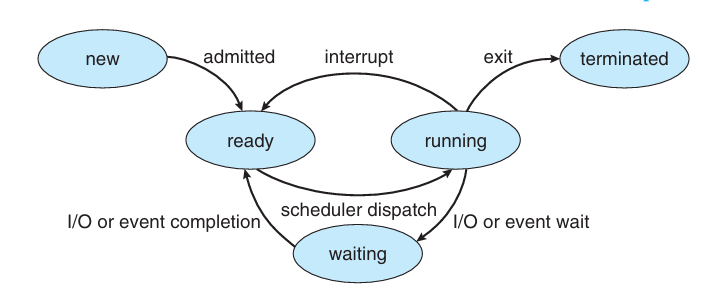
\includegraphics[width=0.92\textwidth]{figures/processstate.png}
    \caption{Các trạng thái của process.}
    \label{fig:processstate}
\end{figure}
Cơ chế lập lịch round-robin của xv6 được định nghĩa trong hàm scheduler() trong file \textit{kernel/proc.c}:
\begin{lstlisting}[caption={scheduler() trong xv6}, language=C]
 for(p = proc; p < &proc[NPROC]; p++) {
      acquire(&p->lock);
      if(p->state == RUNNABLE) {
        p->state = RUNNING;
        c->proc = p;
        swtch(&c->context, &p->context);
        c->proc = 0;
        found = 1;
      }
      release(&p->lock);
    }
\end{lstlisting}
Cơ chế này sẽ quét tất cả 64 process, sau đó chọn process đầu tiên có trạng thái RUNNABLE và chuyển thành RUNNING, và chạy nó luôn. Ta có thế thấy cơ chế này cũng chẳng round-robin lắm, vì nó luôn tim được process đâu tiên ở 
trạng thái RUNNABLE và chạy nó luôn,  tính "round" ở đây chỉ đến việc timer interrupt định kỳ gọi \code{yield()}, trả CPU về scheduler rồi quét lại từ đầu. Ta có thể thấy là nếu tiến trình đọc/ghi ở cuối thì sẽ khó có thể 
được chạy nếu có nhiều tiến trình khác ở trạng thái RUNNABLE mà có index nhỏ hơn index của tiên trình đọc/ghi, trong khi đó các tiến trình đọc, ghi ở trạng thái RUNNABLE nhiều lần khi đọc, ghi một dữ liệu lớn. \\


Việc thực thi tiến trình bao gồm 1 chu kỳ luân phiên giữa thực thi CPU (CPU execution) và đợi I/O (I/O wait) cùng với một khoảng thời gian thực thi là CPU burst và I/O burst, các CPU burst cần một thời gian dài hơn các I/O burst và các lần gọi \code{sleep()} và \code{wakeup()} đều là CPU bound. \\
Do đó, để tăng băng thông, thay vì để reader/writer phải chờ được quét trong scheduler() thì ta sẽ dùng cơ chế lập lịch là sử dụng nhiều hàng đợi ưu tiên (Multilevel Feedback Queue Scheduling), đua ưu tiên của reader/writer là cao nhất.
\begin{figure}[H]
\centering
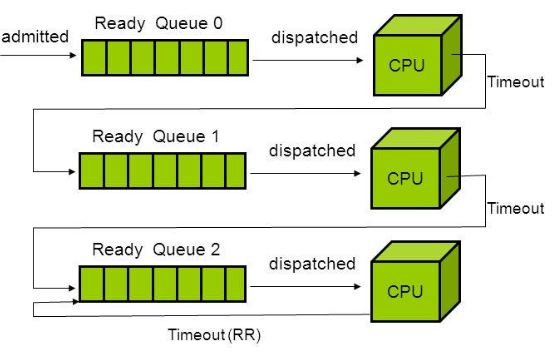
\includegraphics[width=0.92\textwidth]{figures/multilevelfeedback.png}
\caption{Multi-Level Feedback Queue (MLFQ).}
\label{fig:mlfq}
\end{figure}
Cơ chế này phân loại tiến trình dựa trên mỗi lần gọi wakeup(), thì sẽ đặt mức ưu tiên lên cao nhất, do đó nó sẽ luôn được gọi mỗi khi xong 1 tiến trình nào đó, tuy nhiên để tránh 
starvation, mỗi khi timer interrupt gọi \code{yield()}, thì sẽ giảm mức ưu tiên của tiến trình đang ở trạng thái RUNNING, để cho các tiến trình khác có thể chạy, thay vì chỉ chạy wakeup() cho reader/writer. \\

Source code cho version này:
\begin{lstlisting}[caption={v6 -- Priority boost trong wakeup() và scheduler}, language=C]
// kernel/proc.h
#if PIPE_VERSION >= 6
#define PRIORITY_BASE  0
#define PRIORITY_BOOST 10
struct proc {
    // them truong priority vao
    int priority;   // 0 = binh thuong, 10 = boost
};
#endif

// kernel/proc.c -- wakeup() gan priority cao nhat:
if (p->state == SLEEPING && p->chan == chan) {
    p->state = RUNNABLE;
#if PIPE_VERSION >= 6
    p->priority = PRIORITY_BOOST;  // dat priority cao nhat
#endif
}

// scheduler() -- chon process co priority cao nhat:
struct proc *best = 0;
int best_priority = -1;

for(p = proc; p < &proc[NPROC]; p++) {
    if(p->state == RUNNABLE && p->priority > best_priority) {
        best = p;
        best_priority = p->priority;
    }
}

if(best) {
    acquire(&best->lock);
    if(best->state == RUNNABLE) {
        best->state = RUNNING;
        c->proc = best;
        swtch(&c->context, &best->context);
        c->proc = 0;
    }
    release(&best->lock);
}
// yield() -- giam priority moi tick de tranh starvation:
#if PIPE_VERSION >= 6
if (p->priority > PRIORITY_BASE)
    p->priority--;  // giam 1 don vi
#endif
\end{lstlisting}

\textbf{Phân tích code}:
\begin{itemize}\tightlist
    \item[+] Ta thêm một trường \code{priority} vào struct proc để track mức ưu tiên của mỗi process. Mức ưu tiên cơ bản là 0, khi được mức ưu tiên cao nhất là 10.
    \item[+] Trong wakeup(), khi đánh thức một process,ta chuyển trạng thái của nó từ SLEEPING sang RUNNABLE, và đặt mức ưu tiên của nó lên cao nhất (10) để đảm bảo nó được scheduler chọn chạy ngay sau đó.
    \item[+] Trong scheduler(), thay vì chọn process đầu tiên có trạng thái RUNNABLE, 
    ta quét tất cả các process để tìm process có mức ưu tiên cao nhất và chuyển nó từ trạng thái RUNNABLE sang RUNNING.
    \item[+] Trong yield(), mỗi khi timer interrupt gọi yield(), ta giảm mức ưu tiên của process đang chạy xuống 1 đơn vị để tránh starvation, đảm bảo các process khác cũng có cơ hội được chạy.
\end{itemize}

\textbf{Kết quả đo đạc v6}:
\begin{table}[H]
\centering
\caption{So sánh throughput v5 vs v6 (B/s)}
\begin{tabular}{rrrr}
\toprule
\textbf{chunk\_bytes} & \textbf{v5 (B/s)} & \textbf{v6 (B/s)} & \textbf{Tăng} \\
\midrule
64   & 998,643   & 1,048,576  & $1.05\times$ \\
256  & 3,226,387 & 3,495,253  & $1.08\times$ \\
512  & 5,242,880 & 5,242,880  & $1.00\times$ \\
1024 & 6,990,506 & 8,388,608  & $1.20\times$ \\
2048 & 8,388,608 & 10,485,760 & $1.25\times$ \\
\textbf{4096} & \textbf{8,388,608} & \textbf{10,485,760} & $\boldsymbol{1.25\times}$ \\
\bottomrule
\end{tabular}
\end{table}

\textbf{Nhận xét:}
\begin{itemize}
    \item[+] Speedup lớn nhất ở chunk\_bytes lớn (1024--4096) vì đây là kích thước
mà số lần sleep/wakeup nhiều nhất và scheduler delay ảnh hưởng nhiều nhất. Ở chunk\_bytes = 64, pipe hiếm khi đầy nên reader ít khi ngủ $\to$ boost có ít cơ hội.
    \item[+] Cơ chế này chỉ ưu tiên cho wakeup() của reader/writer, do đó nếu reader/writer được đọc/ghi với một chunk\_bytes lớn thi rất hay đầy, và gọi wakeup() liên tục, wakeup() này được 
    gọi liên tục, dẫn đến các tiến trình khác bị bỏ rơi và chỉ được chạy khi đã đọc/ghi hết dữ liệu. 
\end{itemize}


\subsection{v7 -- Cache-line Alignment}

Trong struct pipe của v1--v6, \code{nwrite} và \code{nread} nằm cạnh nhau trong memory,
thường trên cùng một cache line 64~byte. Trong môi trường multi-core
(CPUS $\geq 2$), điều này gây \textbf{false sharing}, do hai hoặc nhiều luồng chạy trên các lõi 
CPU khác nhau cùng cập nhật các biến hoàn toàn độc lập, nhưng các biến này lại nằm cùng một cache line. \\

\textbf{MESI Protocol}: là một giao thức đồng nhất bộ nhớ cache, được sử dụng trong các 
kiến trúc đa xử lý đối xứng SMP. Mục đích của MESI là đảm bảo rằng khi nhiều lõi CPU cùng chia sẻ bộ nhớ chính 
(RAM) nhưng lại sở hữu bộ nhớ cache (L1, L2) độc lập, câc lõi này luôn nhìn thấy một phiên bản nhất quán của dữ liệu, tránh tình trạng đọc phải dữ liệu rác hoặc dữ 
liệu đã cũ. MESI định nghĩa 4 trạng thái mà một cache line có thể có:
\begin{itemize}
    \item \textbf{Modified (M)}: Cache line đã được sửa đổi và chỉ tồn tại trong cache của một lõi CPU. 
    Dữ liệu này chưa được ghi trở lại bộ nhớ chính.
    \item \textbf{Exclusive (E)}: Cache line tồn tại trong cache của một lõi CPU và chưa được sửa đổi. 
    Dữ liệu này là duy nhất trong cache của lõi đó, nhưng đã được ghi trở lại bộ nhớ chính.
    \item \textbf{Shared (S)}: Cache line tồn tại trong cache của một hoặc nhiều lõi CPU và chưa được sửa đổi. 
    Dữ liệu này có thể được chia sẻ giữa các lõi, nhưng không có lõi nào sở hữu quyền sửa đổi.
    \item \textbf{Invalid (I)}: Cache line không hợp lệ hoặc đã bị xóa. 
    Khi một lõi CPU muốn truy cập dữ liệu trên cache line này, nó sẽ phải tải lại dữ liệu từ bộ nhớ chính hoặc từ cache của một lõi khác.
\end{itemize}
Giả sử Core 0 (writer) và Core 1 (reader) chạy song song trên hai lõi khác nhau, cùng truy cập struct pipe với nwrite và nread nằm trên cùng một cache line:
\begin{itemize}\tightlist
    \item Core 0 ghi nwrite $\to$ cache line đó trở thành Modified (M) trong cache của Core 0, và bị Invalid (I) trong cache của Core 1.
    \item Core 1 đọc nread $\to$ cache line đó bị cache miss vì nó đang ở trạng thái Invalid (I) trong cache của Core 1. Core 1 phải gửi yêu cầu đến bộ nhớ chính hoặc cache của Core 0 để lấy dữ liệu mới nhất, dẫn đến stall và phải chờ Core 1 ghi xong.
\end{itemize}

Do đó để tránh false sharing, ta cần tách nwrite và nread ra khỏi cùng một cache line, bằng cách thêm padding để đảm bảo chúng nằm trên các cache line riêng biệt. \\
\textbf{Cấu trúc struct pipe v7 sau padding}:
\begin{lstlisting}[caption={v7 -- Padding 64-byte tách nwrite và nread lên cache line riêng}, language=C]
#if PIPE_VERSION >= 7
#define CACHELINE 64
struct pipe {
  // Cache line 0 (byte 0-63): writer-side
  struct spinlock lock;   // 24 B  \
  char *data;             //  8 B  |  (spinlock: uint+pad+name*+cpu* = 4+4+8+8)
  uint nwrite;            //  4 B  |
  char _pad_w[28];        // 28 B +/  (= 64 - 24 - 8 - 4)
  // Cache line 1 (byte 64-127): reader-side
  uint nread;             //  4 B  \
  char _pad_r[52];        // 52 B +/  (= 64 - 4 - 4 - 4)
  // Cache line 2 (byte 128+): rarely-changed flags
  int  readopen;          //  4 B  \
  int  writeopen;         //  4 B +/
};
#endif
\end{lstlisting}

\textbf{Kết quả:} Core 0 ghi nwrite $\to$ chỉ dirty cache line 0 $\to$ Core 1 đọc
nread $\to$ cache line 1 vẫn valid $\to$ KHÔNG có stall.

\subsubsection{Nhận xét về kết quả v7 trên single-CPU}

\begin{table}[H]
\centering
\caption{So sánh throughput v6 vs v7 (B/s) -- single-CPU}
\begin{tabular}{rrrr}
\toprule
\textbf{chunk\_bytes} & \textbf{v6 (B/s)} & \textbf{v7 (B/s)} & \textbf{Thay đổi} \\
\midrule
64   & 1,048,576  & 1,023,000  & $-2.4\%$ \\
256  & 3,495,253  & 3,495,253  & $0\%$ \\
1024 & 8,388,608  & 8,388,608  & $0\%$ \\
4096 & 10,485,760 & 10,485,760 & $0\%$ \\
\bottomrule
\end{tabular}
\end{table}

Cache-line alignment chỉ phát huy tác dụng rõ khi có từ 2 core trở lên.
Bảng dưới so sánh throughput v7 trên CPUS=1 và CPUS=2:

\begin{table}[H]
\centering
\caption{Throughput v7 (B/s) -- CPUS=1 vs CPUS=2}
\begin{tabular}{rrrr}
\toprule
\textbf{chunk\_bytes} & \textbf{CPUS=1 (B/s)} & \textbf{CPUS=2 (B/s)} & \textbf{Tăng} \\
\midrule
64   & 1,023,000  & 1,271,001  & $+24.2\%$ \\
256  & 3,495,253  & 3,495,253  & $0\%$ \\
1024 & 8,388,608  & 8,388,608  & $0\%$ \\
4096 & 10,485,760 & 20,971,520 & $+100\%$ \\
\bottomrule
\end{tabular}
\end{table}


\subsection{v8 -- All Combined (Tổng hợp tất cả cơ chế v2--v7)}

\subsubsection{Mục tiêu -- Kết hợp 5 cơ chế thành 1 phiên bản hoàn chỉnh}

Sau khi phân tích 7 phiên bản, nhóm xác định 5 cơ chế tối ưu không xung đột nhau và
kết hợp tất cả vào v8. v8 không thêm kỹ thuật mới -- mục tiêu là có một phiên bản
duy nhất chứa đầy đủ toàn bộ cải tiến::

\begin{table}[H]
\centering
\caption{5 cơ chế được kết hợp trong v8}
\begin{tabular}{clll}
\toprule
\textbf{\#} & \textbf{Cơ chế} & \textbf{Nguồn gốc} & \textbf{Bottleneck giải quyết} \\
\midrule
1 & Bulk copyin/copyout & v2 & $n$ lần page walk $\to$ $\leq 2$/write \\
2 & Trang dữ liệu riêng (4~KB) & v4 & metadata và data tách biệt \\
3 & Lazy wakeup & v5 & $O(\text{NPROC})$ wakeup $\to O(1)$ \\
4 & Priority boost & v6 & scheduler delay sau wakeup \\
5 & Cache-line alignment & v7 & false sharing trên multi-core \\
\bottomrule
\end{tabular}
\end{table}

\subsubsection{Thiết kế v8}

v8 dùng lại toàn bộ \code{struct pipe} và logic của v7:

\begin{lstlisting}[caption={v8 -- struct pipe và PIPE\_TOTAL giống v7}, language=C]
#define DATA_PAGES 1
#define PIPE_TOTAL (DATA_PAGES * PGSIZE)   // 4096 byte
#define CACHELINE  64

struct pipe {
  // Cache line 0 (byte 0-63): writer-side
  struct spinlock lock;   // 24 B
  char *data;             //  8 B  -- 1 trang kalloc rieng
  uint nwrite;            //  4 B
  char _pad_w[28];        // 28 B  (= 64 - 24 - 8 - 4)
  // Cache line 1 (byte 64-127): reader-side
  uint nread;             //  4 B
  char _pad_r[52];        // 52 B
  // Cache line 2: rarely-changed flags
  int  readopen;
  int  writeopen;
};
\end{lstlisting}

\subsubsection{Kết quả benchmark -- v1 vs v8}

\begin{table}[H]
\centering
\small
\caption{So sánh throughput v1 vs v8 -- CPUS=1 và CPUS=2 (B/s)}
\begin{tabular}{rrrrrrr}
\toprule
& \multicolumn{3}{c}{\textbf{CPUS = 1}} & \multicolumn{3}{c}{\textbf{CPUS = 2}} \\
\cmidrule(lr){2-4}\cmidrule(lr){5-7}
\textbf{chunk} & \textbf{v1} & \textbf{v8} & \textbf{Speedup} & \textbf{v1} & \textbf{v8} & \textbf{Speedup} \\
\midrule
64   & 198,782 & 1,023,000  & $5.15\times$ & 236,966 & 1,353,001  & $5.71\times$ \\
256  & 419,430 & 3,495,253  & $8.33\times$ & 505,337 & 3,495,253  & $6.92\times$ \\
1024 & 511,500 & 8,388,608  & $16.4\times$ & 655,360 & 6,990,506  & $10.7\times$ \\
4096 & 559,240 & 13,981,013 & $25.0\times$ & 710,898 & 13,981,013 & $19.7\times$ \\
\bottomrule
\end{tabular}
\end{table}

% ===========================================================================
\section{Source Code Review -- v8}
\label{sec:code}
% ===========================================================================

Phần này trình bày source code đầy đủ của \textbf{v8} -- phiên bản tổng hợp tất cả
cải tiến từ v2 đến v7. Bốn hàm chính: \code{pipealloc}, \code{pipeclose},
\code{pipewrite}, \code{piperead}.

\subsection{pipealloc()}

\code{pipealloc()} cấp phát \textbf{2 trang vật lý} riêng biệt: trang 1 chứa
\code{struct pipe} (metadata + cache-line padding), trang 2 chứa data buffer 4096~byte.

\begin{lstlisting}[caption={pipealloc() -- v8: 2 trang rieng biet (kernel/pipe.c)},
                   language=C]
int
pipealloc(struct file **f0, struct file **f1)
{
  struct pipe *pi;

  pi = 0;
  *f0 = *f1 = 0;
  if((*f0 = filealloc()) == 0 || (*f1 = filealloc()) == 0)
    goto bad;
  if((pi = (struct pipe*)kalloc()) == 0)   // trang 1: struct pipe
    goto bad;
  if((pi->data = (char*)kalloc()) == 0){   // trang 2: data buffer 4096 B
    kfree((char*)pi);
    pi = 0;
    goto bad;
  }
  pi->readopen  = 1;
  pi->writeopen = 1;
  pi->nwrite    = 0;
  pi->nread     = 0;
  initlock(&pi->lock, "pipe");
  (*f0)->type = FD_PIPE;
  (*f0)->readable = 1;
  (*f0)->writable = 0;
  (*f0)->pipe = pi;
  (*f1)->type = FD_PIPE;
  (*f1)->readable = 0;
  (*f1)->writable = 1;
  (*f1)->pipe = pi;
  return 0;

 bad:
  if(pi)
    kfree((char*)pi);
  if(*f0)
    fileclose(*f0);
  if(*f1)
    fileclose(*f1);
  return -1;
}
\end{lstlisting}

\subsection{pipeclose()}

\code{pipeclose()} đánh dấu đầu đóng, đánh thức đầu kia, và giải phóng bộ nhớ
khi cả hai đầu đã đóng. v8 cần \code{kfree} đúng 2 lần: data page trước, struct page sau.

\begin{lstlisting}[caption={pipeclose() -- v8: giai phong 2 trang (kernel/pipe.c)},
                   language=C]
void
pipeclose(struct pipe *pi, int writable)
{
  acquire(&pi->lock);
  if(writable){
    pi->writeopen = 0;
    wakeup(&pi->nread);    // wake reader: writer end closed
  } else {
    pi->readopen = 0;
    wakeup(&pi->nwrite);   // wake writer: reader end closed
  }
  if(pi->readopen == 0 && pi->writeopen == 0){
    release(&pi->lock);
    kfree(pi->data);       // free data page first
    kfree((char*)pi);      // then free struct page
  } else
    release(&pi->lock);
}
\end{lstlisting}

\subsection{pipewrite()}

\code{pipewrite()} ghi dữ liệu từ user space vào pipe buffer. v8 dùng:
\textbf{(1)} bulk \code{copyin} thay byte-by-byte,
\textbf{(2)} lazy wakeup -- chỉ gọi \code{wakeup(\&pi->nread)} khi buffer thực sự
rỗng lúc bắt đầu ghi.

\begin{lstlisting}[caption={pipewrite() -- v8: bulk copy + lazy wakeup (kernel/pipe.c)},
                   language=C]
int
pipewrite(struct pipe *pi, uint64 addr, int n)
{
  int i = 0;
  struct proc *pr = myproc();

  acquire(&pi->lock);
  // buffer empty at entry -> reader may be sleeping -> need wakeup later
  int need_wakeup = (pi->nwrite == pi->nread);

  while(i < n){
    if(pi->readopen == 0 || killed(pr)){
      release(&pi->lock);
      return -1;
    }
    if(pi->nwrite == pi->nread + PIPE_TOTAL){
      wakeup(&pi->nread);              // mandatory before sleep
      sleep(&pi->nwrite, &pi->lock);
      need_wakeup = 1;                 // after waking up, reader may have re-slept
    } else {
      uint free_slots = PIPE_TOTAL - (pi->nwrite - pi->nread);
      uint head_slot  = pi->nwrite % PIPE_TOTAL;
      uint till_wrap  = PIPE_TOTAL - head_slot; // bytes left before ring wrap
      int to_copy = (int)umin((uint)(n - i), umin(free_slots, till_wrap));
      if(copyin(pr->pagetable, &pi->data[head_slot], addr + i, to_copy) == -1)
        break;
      pi->nwrite += to_copy;
      i          += to_copy;
    }
  }
  if(need_wakeup && i > 0)
    wakeup(&pi->nread);    // skip wakeup on fast path (reader still running)
  release(&pi->lock);
  return i;
}
\end{lstlisting}

\subsection{piperead()}

\code{piperead()} đọc dữ liệu từ pipe buffer ra user space. v8 dùng lazy wakeup đối
xứng: chỉ gọi \code{wakeup(\&pi->nwrite)} khi buffer \emph{đã đầy} lúc bắt đầu đọc
-- lúc đó writer mới có thể đang ngủ.

\begin{lstlisting}[caption={piperead() -- v8: bulk copy + lazy wakeup (kernel/pipe.c)},
                   language=C]
int
piperead(struct pipe *pi, uint64 addr, int n)
{
  int i = 0;
  struct proc *pr = myproc();

  acquire(&pi->lock);
  // wait until data is available or writer has closed
  while(pi->nread == pi->nwrite && pi->writeopen){
    if(killed(pr)){
      release(&pi->lock);
      return -1;
    }
    sleep(&pi->nread, &pi->lock);
  }
  // buffer full at entry -> writer may be sleeping -> need wakeup later
  int was_full = (pi->nwrite == pi->nread + PIPE_TOTAL);

  while(i < n){
    if(pi->nread == pi->nwrite)
      break;
    uint avail     = pi->nwrite - pi->nread;
    uint tail_slot = pi->nread % PIPE_TOTAL;
    uint till_wrap = PIPE_TOTAL - tail_slot;  // bytes left before ring wrap
    int to_copy = (int)umin((uint)(n - i), umin(avail, till_wrap));
    if(copyout(pr->pagetable, addr + i, &pi->data[tail_slot], to_copy) == -1){
      if(i == 0) i = -1;
      break;
    }
    pi->nread += to_copy;
    i         += to_copy;
  }
  if(was_full && i > 0)
    wakeup(&pi->nwrite);   // skip wakeup on fast path (writer still running)
  release(&pi->lock);
  return i;
}
\end{lstlisting}




% ===========================================================================
\section{Phân tích tổng thể}
\label{sec:analysis}
% ===========================================================================

\subsection{Định luật Amdahl}
\textbf{Định luật Amdahl:} Cho $p$ là phần chi phí có thể tối ưu (``parallelizable
fraction''), $s$ là speedup của phần đó sau khi tối ưu:
\begin{equation}
\text{Speedup}(s) = \frac{1}{(1-p) + p/s}
\end{equation}
Khi $s \to \infty$ (tối ưu phần $p$ hoàn toàn): $\text{Speedup}_{\max} = \frac{1}{1-p}$.

Để áp dụng Định luật Amdahl, cần xác định $p$ -- tỉ lệ chi phí \textbf{có thể tối ưu}
trong tổng chi phí của v1. Từ phân tích v1 ở \S\ref{sec:baseline}, mỗi lần ghi
$n = 4096$~byte qua pipe tốn:

\begin{table}[H]
\centering
\caption{Phân rã chi phí v1 -- $n = 4096$~byte, QEMU single-CPU}
\label{tab:cost_breakdown}
\begin{tabular}{lrr}
\toprule
\textbf{Thành phần} & \textbf{Cycle ước tính} & \textbf{\%} \\
\midrule
$4096 \times$ \code{copyin}(1B), $\approx 80$c/lần
  & $\sim 327{,}680$ & $\sim 74\%$ \\
$4096 \times$ lock acquire/release, $\approx 20$c/lần
  & $\sim 81{,}920$ & $\sim 9\%$ \\
Scheduler delay (reader chờ được lập lịch)
  & $\sim$ nhiều & $\sim 13\%$ \\
$8 \times$ sleep/wakeup $\approx 2000$c/lần
  & $\sim 16{,}000$ & $\sim 2\%$ \\
$4096 \times$ kiểm tra điều kiện + branch
  & $\sim 20{,}000$ & $\sim 2\%$ \\
\midrule
\textbf{Tổng có thể tối ưu} & & $\approx \mathbf{97\%}$ \\
\midrule
Syscall trap path (cố định, không thể bỏ)
  & $\sim 400$ & $\sim 0.1\%$ \\
Lock overhead tối thiểu (không thể bỏ)
  & $\sim$ nhỏ & $\sim 3\%$ \\
\midrule
\textbf{Tổng không thể tối ưu} $(1-p)$ & & $\approx \mathbf{3\%}$ \\
\bottomrule
\end{tabular}
\end{table}

\textbf{Cách suy luận:}
\begin{itemize}\tightlist
  \item Thành phần lớn nhất -- \textbf{74\% chi phí copyin/copyout} -- đến từ việc v1
  gọi \code{copyin()} đúng $n$ lần, mỗi lần dịch địa chỉ qua page table
  (\code{walkaddr}) rồi copy 1~byte. Đây hoàn toàn có thể tối ưu bằng bulk copy.
  \item \textbf{13\% scheduler delay}: sau mỗi \code{wakeup()}, reader trở thành
  RUNNABLE nhưng round-robin scheduler không chọn nó ngay -- CPU nhàn rỗi hoặc
  chạy process khác. Tối ưu bằng priority boost (v6).
  \item \textbf{9\% lock overhead}: phần lớn là \code{mfence}/\code{amoswap} của
  spinlock -- không thể bỏ hoàn toàn (mutual exclusion bắt buộc), nhưng giảm được
  false sharing bằng cache-line alignment (v7).
  \item \textbf{Phần không thể tối ưu $(1-p) \approx 3\%$}: syscall trap path
  (ecall $\to$ usertrap $\to$ sret) là chi phí cố định mỗi lần \code{write()}/\code{read()},
  không phụ thuộc vào pipe implementation.
\end{itemize}

Do đó: $p \approx 1 - 0.03 = 0.97$.

\subsubsection{Áp dụng Định luật Amdahl}

Từ cost model của v1: $p \approx 0.97$ (97\% chi phí có thể tối ưu).
\begin{equation}
\text{Speedup}_{\max}(p=0.97) = \frac{1}{1-0.97} = \frac{1}{0.03} \approx 33\times
\end{equation}

\textbf{Đo thực tế:} Speedup(v8/v1) = $20.9\times$ tại chunk\_bytes = 4096.

Thực tế \textbf{nằm trong dự đoán} ($20.9 < 33$) và phù hợp với Định luật Amdahl.
Khoảng cách giữa giới hạn lý thuyết ($33\times$) và thực tế ($20.9\times$) đến từ
phần chi phí không thể tối ưu (overhead syscall, trap path, spinlock) và thực tế
v8 không tăng buffer như kế hoạch ban đầu.


\subsection{Bài học kinh nghiệm (Methodology)}

\begin{enumerate}
    \item \textbf{``Measure first, optimize second'':} Phân tích baseline kỹ lưỡng
    (12 yếu tố, cost model, đo rdcycle trực tiếp) giúp xác định đúng bottleneck.
    Nhóm dành nguyên Tuần 5 chỉ để phân tích v1 trước khi viết bất kỳ tối ưu nào.
    Kết quả: mỗi optimization chính xác, không ``tối ưu mù''.

    \item \textbf{Mỗi version, một bottleneck:} Mỗi bước cải tiến chỉ nhắm vào một
    bottleneck đã được đo, giúp đánh giá chính xác đóng góp của từng kỹ thuật. Ablation
    study v2-cap2048 minh họa tầm quan trọng của việc kiểm soát biến.

    \item \textbf{Trade-off là thực:} v7 (cache-line alignment) chậm hơn v6 trên
    single-CPU vì struct lớn hơn -- đây là kết quả đúng, không phải bug. Tối ưu cho
    multi-core có thể gây hại single-core. Hiểu rõ điều này là quan trọng để không
    vội kết luận sai.

    \item \textbf{Lý thuyết dự đoán thực tế:} Cost model (Amdahl, Producer-Consumer,
    MESI, MLFQ scheduling) giúp dự đoán kết quả trước khi đo. Sai lệch 3--5\% giữa
    dự đoán và thực đo xác nhận model đủ tốt để xếp hạng tương đối.

    \item \textbf{Benchmark phải công bằng:} Dùng cùng \code{pipebench.c} trên cùng
    môi trường (QEMU CPUS=1, cùng total\_bytes = 4MB, cùng dải chunk\_bytes) cho tất cả
    phiên bản là điều kiện cần thiết để so sánh có ý nghĩa.

    \item \textbf{Kernel space vs User space:} Triển khai tối ưu ở kernel space
    (sửa \code{kernel/pipe.c}, \code{kernel/proc.c}, \code{kernel/proc.h}) thay vì user
    space giúp đạt hiệu quả thực sự -- user space không thể thay đổi bộ đệm pipe, lịch
    trình CPU, hay cơ chế sleep/wakeup.
\end{enumerate}


\subsection{Hạn chế và hướng mở rộng}

\textbf{Hạn chế hiện tại:}
\begin{itemize}\tightlist
    \item Toàn bộ benchmark chạy trên QEMU CPUS=1. v7 (cache-line alignment) cần đo
    lại với CPUS=2 để xác nhận lợi ích thực trong môi trường multi-core.
    \item Chưa đo throughput với workload bất đối xứng (writer nhanh hơn reader nhiều lần).
\end{itemize}

\textbf{Hướng mở rộng tiềm năng:}
\begin{itemize}\tightlist
    \item \textbf{Zero-copy:} Thay vì copyin/copyout qua kernel buffer, map trực tiếp
    page của user process vào pipe $\to$ loại bỏ hoàn toàn chi phí copy. Đây là kỹ
    thuật được dùng trong \code{splice()} và \code{sendfile()} của Linux.
    \item \textbf{Lock-free ring buffer:} Dùng atomic operations thay spinlock để loại
    bỏ hoàn toàn lock contention trong single-producer/single-consumer case.
\end{itemize}

% ===========================================================================
% ===========================================================================
\begin{thebibliography}{9}

\bibitem{silberschatz2018}
Abraham Silberschatz, Peter B. Galvin, Greg Gagne.
\textit{Operating System Concepts}, 10th Edition.
Wiley, 2018.

\bibitem{xv6riscv}
Russ Cox, Frans Kaashoek, Robert Morris.
\textit{xv6: a simple, Unix-like teaching operating system}.
MIT, 2023.
\url{https://pdos.csail.mit.edu/6.828/2023/xv6/book-riscv-rev3.pdf}

\end{thebibliography}

\end{document}
